\chapter{Swiss Terrain 3D}
\label{chap_swiss_terrain_3d}
Kapitel \ref{chap_datengrundlage} behandelte die Datengrundlage für die Terrainvisualisierung. In Kapitel \ref{chap_technologien} wurden Programme und Frameworks zur Erstellung von 3D-Visualisierungen thematisiert. Die technisch notwendigen Grundlagen zur Grafikprogrammierung wurden im Rahmen von Kapitel \ref{chap_render_pipelines} erläutert. Kapitel \ref{chap_algorithmen} befasste sich mit gängigen Datenstrukturen und Algorithmen. Aufbauend auf diesem Vorwissen geht es in diesem Kapitel nun um die eigentliche Implementierung der Terrainvisualisierung.

\section{Technologie und Anforderungen}
\label{technologie_anforderungen}
Bevor mit der Implementierung einer Visualisierung begonnen werden kann, müssen sowohl die Anforderungen als auch die eingesetzte Technologie definiert werden. Eine echtzeitfähige 3D-Visualisierung ist vereinfacht ausgedrückt eine fortlaufende Abfolge von Bildern, die von der Grafikkarte erzeugt werden. Die Bildgenerierung erfolgt dabei unter Berücksichtigung von Parametern wie Kameraperspektive, Datenbasis und Interaktion. Damit eine Visualisierung als echtzeitfähig gilt, wird in der Regel eine Bildrate von mindestens 30 Bildern pro Sekunde (FPS) vorausgesetzt. Moderne Monitore unterstützen jedoch deutlich höhere Bildfrequenzen, sodass Darstellungsraten von 60 bis 140 FPS inzwischen weit verbreitet sind. Neben der Bildrate spielt auch die Auflösung eine entscheidende Rolle. Je höher die Auflösung, desto detailgetreuer lässt sich die Visualisierung darstellen. Sowohl eine hohe Auflösung als auch eine hohe Bildrate erfordern eine entsprechend leistungsfähige Grafikkarte, was den Kreis der potenziellen Zielgruppe einschränken kann. Um einen ausgewogenen Kompromiss zwischen visueller Qualität und breiter Nutzbarkeit zu erreichen, legt diese Masterarbeit daher folgende Mindestanforderung an die Visualisierung fest:\textit{Die Visualisierung soll mit mindestens 60 Bildern pro Sekunde bei einer Auflösung von 2k laufen}.

Neben den technischen Anforderungen stellt sich auch die Frage, welche Plattformen unterstützt werden sollen. Auf den meisten Betriebssystemen sowie mobilen Endgeräten sind bereits Webbrowser vorinstalliert. Browserbasierte Anwendungen bieten zudem den Vorteil, dass kein zusätzlicher Installationsaufwand erforderlich ist. Um eine möglichst breite Zielgruppe ohne zusätzliche Hürden zu erreichen, wurde daher eine webbasierte Implementierung gewählt.

Wie in Kapitel \ref{chap_technologien} thematisiert, unterstützen moderne Engines wie Unity, Unreal und Godot grundsätzlich auch die Entwicklung browserbasierter Anwendungen. Die primäre Zielplattform dieser Engines sind jedoch nach wie vor native Anwendungen für Desktop- und mobile Endgeräte. Zudem fallen bei kommerziellen Lösungen wie Unity und Unreal entsprechende Lizenzgebühren an. Obwohl Spiele-Engines eine Vielzahl an Werkzeugen bereitstellen, die die Entwicklung von 3D-Anwendungen erleichtern, setzt deren effektive Nutzung eine umfangreiche Einarbeitung voraus. Ebenso sind Engines bei auftretenden technischen Limitationen nur eingeschränkt anpassbar, da der Zugriff auf den Quellcode – insbesondere bei proprietären Lösungen – begrenzt ist. Zusätzlich erfordern Engines wie Unreal eine vergleichsweise leistungsfähige Hardware, um sinnvoll eingesetzt werden zu können. Vor diesem Hintergrund wurde für diese Arbeit ein webbasiertes Framework anstelle einer Spiele-Engine gewählt. Sowohl Three.js als auch Babylon.js unterstützen moderne Grafikschnittstellen wie WebGL2 und WebGPU. Da das CAVE-System der FHGR auf Three.js basiert, fiel die Entscheidung zugunsten von Three.js. Zusätzlich profitiert Three.js von einer grösseren Community sowie einer Vielzahl an frei verfügbaren Beispielanwendungen (siehe Kapitel \ref{chap_technologien}).

\section{Datenvorverarbeitung}
Um eine manuelle Datenvorverarbeitung zu vermeiden, wurden die nachfolgend beschriebenen Schritte weitgehend mithilfe eines Python-Skripts automatisiert. Dadurch entfällt eine manuelle Durchführung der einzelnen Verarbeitungsschritte. Abbildung \ref{fig_data_preprocessing} bietet einen Überblick über den gesamten Datenvorverarbeitungsprozess. Im Folgenden werden die zentralen Teilbereiche näher erläutert.
\begin{figure}[H]
    \caption{Übersicht Datenvorverarbeitung (Eigene Darstellung)}
    \includegraphics[width=.15\linewidth]{content/00_assets/uebersicht_datenvorverarbeitung.png}
    \label{fig_data_preprocessing}
\end{figure}

\subsection{Herunterladen der Daten}
Sowohl der swissALTI3D- als auch der swissIMAGE-Datensatz stehen kostenfrei über die swisstopo-Webseite zum Download bereit (siehe Abbildung \ref{fig_swisstopo_datenbezug}). Zu Beginn wird der gewünschte geografische Bereich definiert. Dies kann durch die Auswahl einer Gemeinde, eines Kantons oder durch das manuelle Festlegen eines Bereichs auf der Karte erfolgen (siehe Bereich A in Abbildung \ref{fig_swisstopo_datenbezug}). Anschliessend werden das gewünschte Datenformat sowie die entsprechende Auflösung ausgewählt (siehe Bereich B in Abbildung \ref{fig_swisstopo_datenbezug}). Daraufhin kann eine CSV-Datei heruntergeladen werden, die eine Sammlung von Download-Links zu den einzelnen Datensätzen enthält. Jeder Datensatz repräsentiert dabei einen geografischen Bereich von einem Quadratkilometer. Diese Bereiche werden im Folgenden als ``Tiles'' bezeichnet. Um die einzelnen Tiles nicht manuell herunterladen zu müssen, wurde ein Python-Skript entwickelt, das die CSV-Datei einliest, die referenzierten Dateien automatisiert herunterlädt und strukturiert in entsprechenden Ordnern ablegt.

\begin{figure}[H]
    \caption{Herunterladen der swisstopo Daten (Eigene Darstellung)}
    \includegraphics[width=.4\linewidth]{content/00_assets/swisstopo_datenauswahl.png}
    \label{fig_swisstopo_datenbezug}
\end{figure}


Die in den CSV-Dateien enthaltenen Download-Links decken nicht in allen Fällen einen vollständig zusammenhängenden geografischen Bereich ab. Wird etwa die Region Sarganserland auf der swisstopo-Webseite ausgewählt und die heruntergeladenen Tiles zu einem Gesamtbild zusammengesetzt, zeigen sich Datenlücken in Form schwarzer Bereiche (siehe Abbildung \ref{fig_swisstopo_daten_luecken}). Da die Datensätze jedoch georeferenziert sind und auf dem LV95-Koordinatensystem basieren, lassen sich diese fehlenden Bereiche identifizieren und entsprechend schliessen (siehe Abbildung \ref{fig_swisstopo_daten_luecken}). 

\begin{figure}[H]
    \caption{Lücken in swisstopo-Daten (links) mit automatischer Korrektur (rechts) (Eigene Darstellung)}
    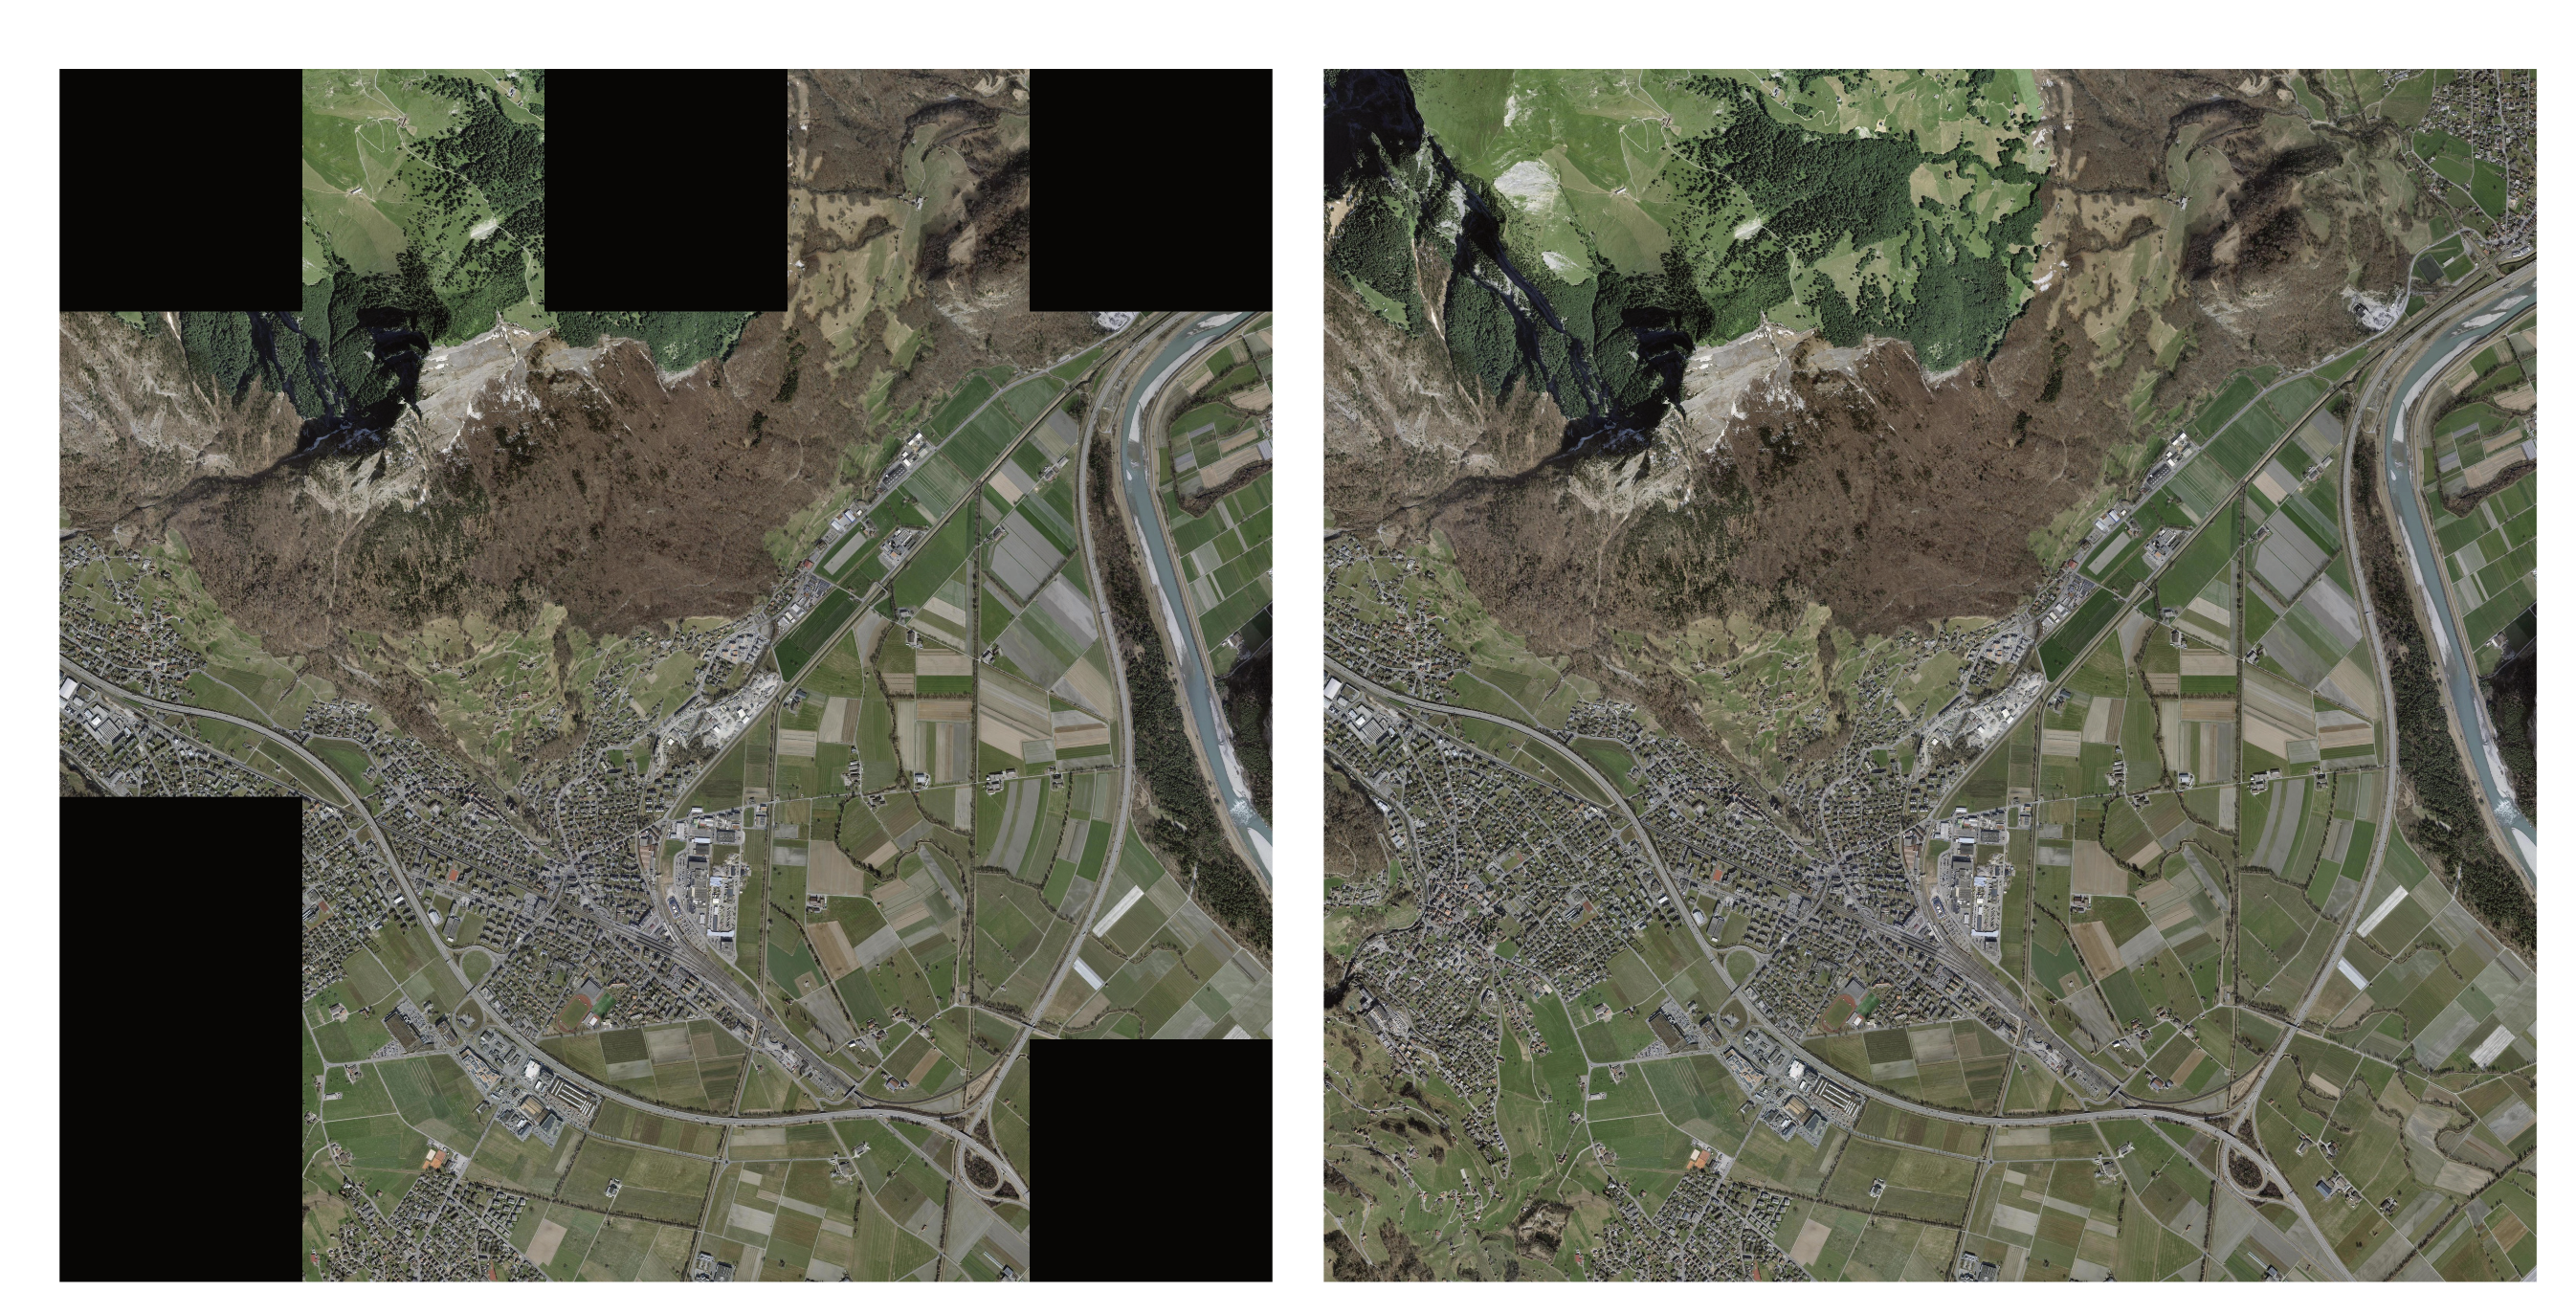
\includegraphics[width=.6\linewidth]{content/00_assets/gesamtbild_mit_luecken.png}
    \label{fig_swisstopo_daten_luecken}
\end{figure}

\subsection{Extrahierung der Höhenwerte und Bilddaten}
Nach dem Herunterladen der Daten werden sowohl die Bildinformationen als auch die Höhendaten aus den GeoTIFF-Dateien extrahiert und als eigenständige Texturen gespeichert. Die Höhenwerte werden dabei in Form eines Graustufenbildes abgelegt, wobei helle Bereiche hohe Höhenwerte und dunkle Bereiche niedrige Höhenwerte repräsentieren (siehe Abbildung \ref{fig_heightmap_beispiel}).

\begin{figure}[H]
    \caption{Extrahierte Höhenwerte als Graustufenbild (Eigene Darstellung)}
    \includegraphics[width=.4\linewidth]{content/00_assets/heightmap_beispiel.png}
    \label{fig_heightmap_beispiel}
\end{figure}

Um die Geopositionsinformationen zu erhalten, werden diese direkt in den Dateinamen der erzeugten Texturen integriert. Da die swisstopo-Daten in Form einzelner Tiles bereitgestellt werden, müssen diese in einem nächsten Schritt zu einem Gesamtbild zusammengesetzt werden. Die Positionierung erfolgt anhand des LV95-Koordinatensystems. Dabei zeigt sich jedoch ein Problem. Jede Tile besitzt einen eigenen minimalen und maximalen Höhenwert. Werden diese ohne weitere Verarbeitung kombiniert, entstehen keine fliessenden Übergänge. Um dieses Problem zu beheben, werden die Höhenwerte aller Tiles mithilfe eines globalen Minimal- und Maximalwertes normalisiert und somit konsistente Übergänge geschaffen (siehe Abbildung \ref{fig_heightmap_sargans}).

\begin{figure}[H]
    \caption{Zusammengesetztes Graustufenbild von Sargans mit fliessenden (links) und nicht fliessenden (rechts) Übergängen (Eigene Darstellung)}
    \includegraphics[width=.7\linewidth]{content/00_assets/heightmap_sargans.png}
    \label{fig_heightmap_sargans}
\end{figure}

Das Extrahieren der Farbwerte aus dem swissIMAGE-Datensatz gestaltet sich vergleichsweise unkompliziert, da lediglich die Farbinformationen aus den Dateien ausgelesen werden müssen und keine zusätzliche Normalisierung erforderlich ist (siehe Abbildung \ref{fig_textur_sargans}). Aufgrund unterschiedlicher Aufnahmezeitpunkte der Luftbilder können jedoch visuelle Diskrepanzen auftreten, wie sie im Bereich A von Abbildung \ref{fig_textur_sargans} zu erkennen sind.

\begin{figure}[H]
    \caption{Zusammengesetztes Luftbild von Sargans (Eigene Darstellung)}
    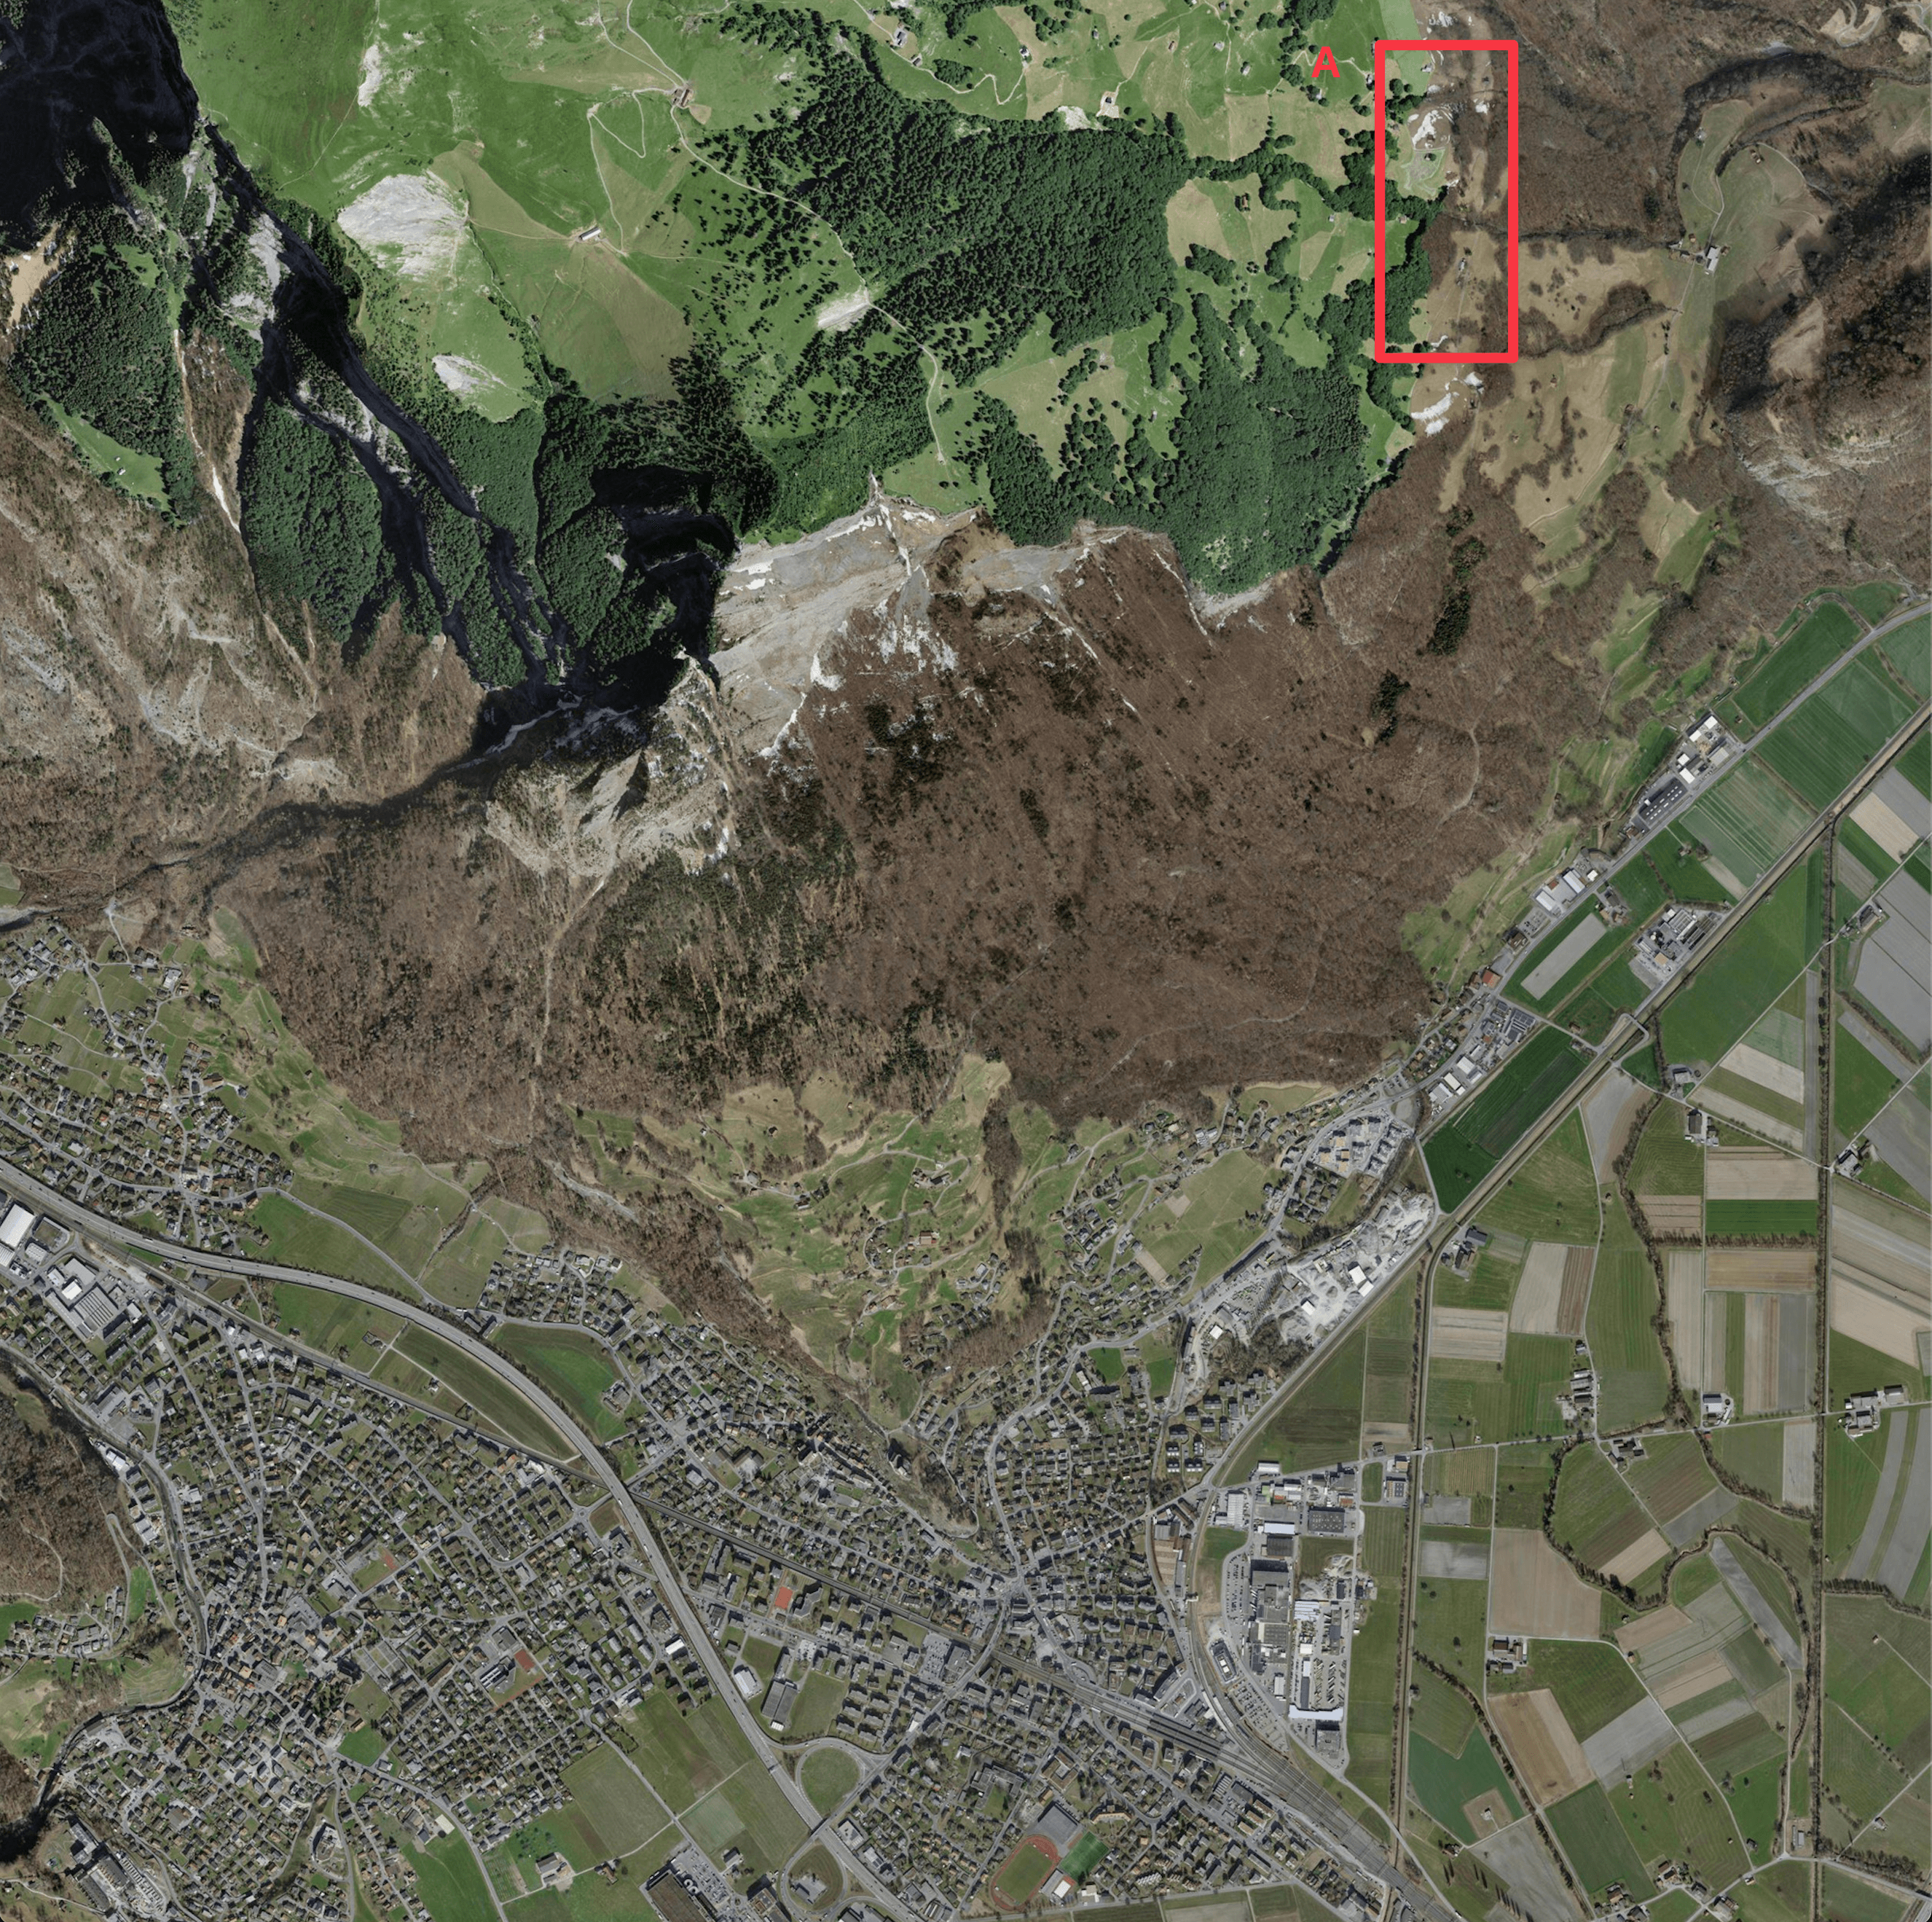
\includegraphics[width=.4\linewidth]{content/00_assets/textur_sargans.png}
    \label{fig_textur_sargans}
\end{figure}

\subsection{Aufteilung in kleinere Bilddateien}
Wie in Kapitel \ref{chap_datengrundlage} beschrieben, variiert der benötigte Festplattenspeicher der swisstopo-Datensätze in Abhängigkeit von Auflösung und geografischem Gebiet. Für die Region Sargans ergibt sich bei der höchsten Auflösung von 10 cm pro Bildpunkt ein zusammengesetztes Luftbild mit einer Grösse von rund 7.5GB. Eine derart grosse Datenmenge ist für eine browserbasierte Anwendung nur eingeschränkt geeignet, da andernfalls mit erheblichen Ladezeiten zu rechnen ist. Zwar bieten browserbasierte Anwendungen den Vorteil, ortsunabhängig nutzbar zu sein, jedoch müssen die erforderlichen Daten zunächst auf das Endgerät übertragen werden. Abhängig von der verfügbaren Internetbandbreite kann dieser Vorgang viel Zeit in Anspruch nehmen. Das vollständige Herunterladen grosser Datenmengen stellt daher – selbst unter Verwendung von Ladeindikatoren – keine skalierbare Lösung dar.

Zur Bewältigung dieser Problematik werden im Rahmen der Datenvorverarbeitung mehrere Schritte durchgeführt. Zunächst wird das Gesamtbild in kleinere Bilddateien aufgeteilt. Um sowohl den Speicherbedarf als auch die Ladezeiten zu verkürzen, werden diese anschliessend mittels eines Downsampling-Algorithmus skaliert.

Die Aufteilung der Bilddaten erfolgt auf Basis des Quadtree-Algorithmus, wobei Tiles in unterschiedlichen Auflösungsstufen (Level of Detail, LOD) erzeugt werden. Die jeweilige Auflösung ist dabei direkt an die Baumtiefe des Quadtrees gekoppelt. Für die erste Auflösung (LOD 1) wird das Gesamtbild in 4 (4$^1$) Tiles aufgeteilt. Für die zweite Auflösung sind es hingegen 16 (4$^2$) etc. Abbildung \ref{fig_textur_teilbilder_quadtree} veranschaulicht die Aufteilung eines Gesamtbildes in Tiles unterschiedlicher Auflösung.
\begin{figure}[H]
    \caption{Aufteilung in Tiles mit unterschiedlichen Auflösungen (Eigene Darstellung)}
    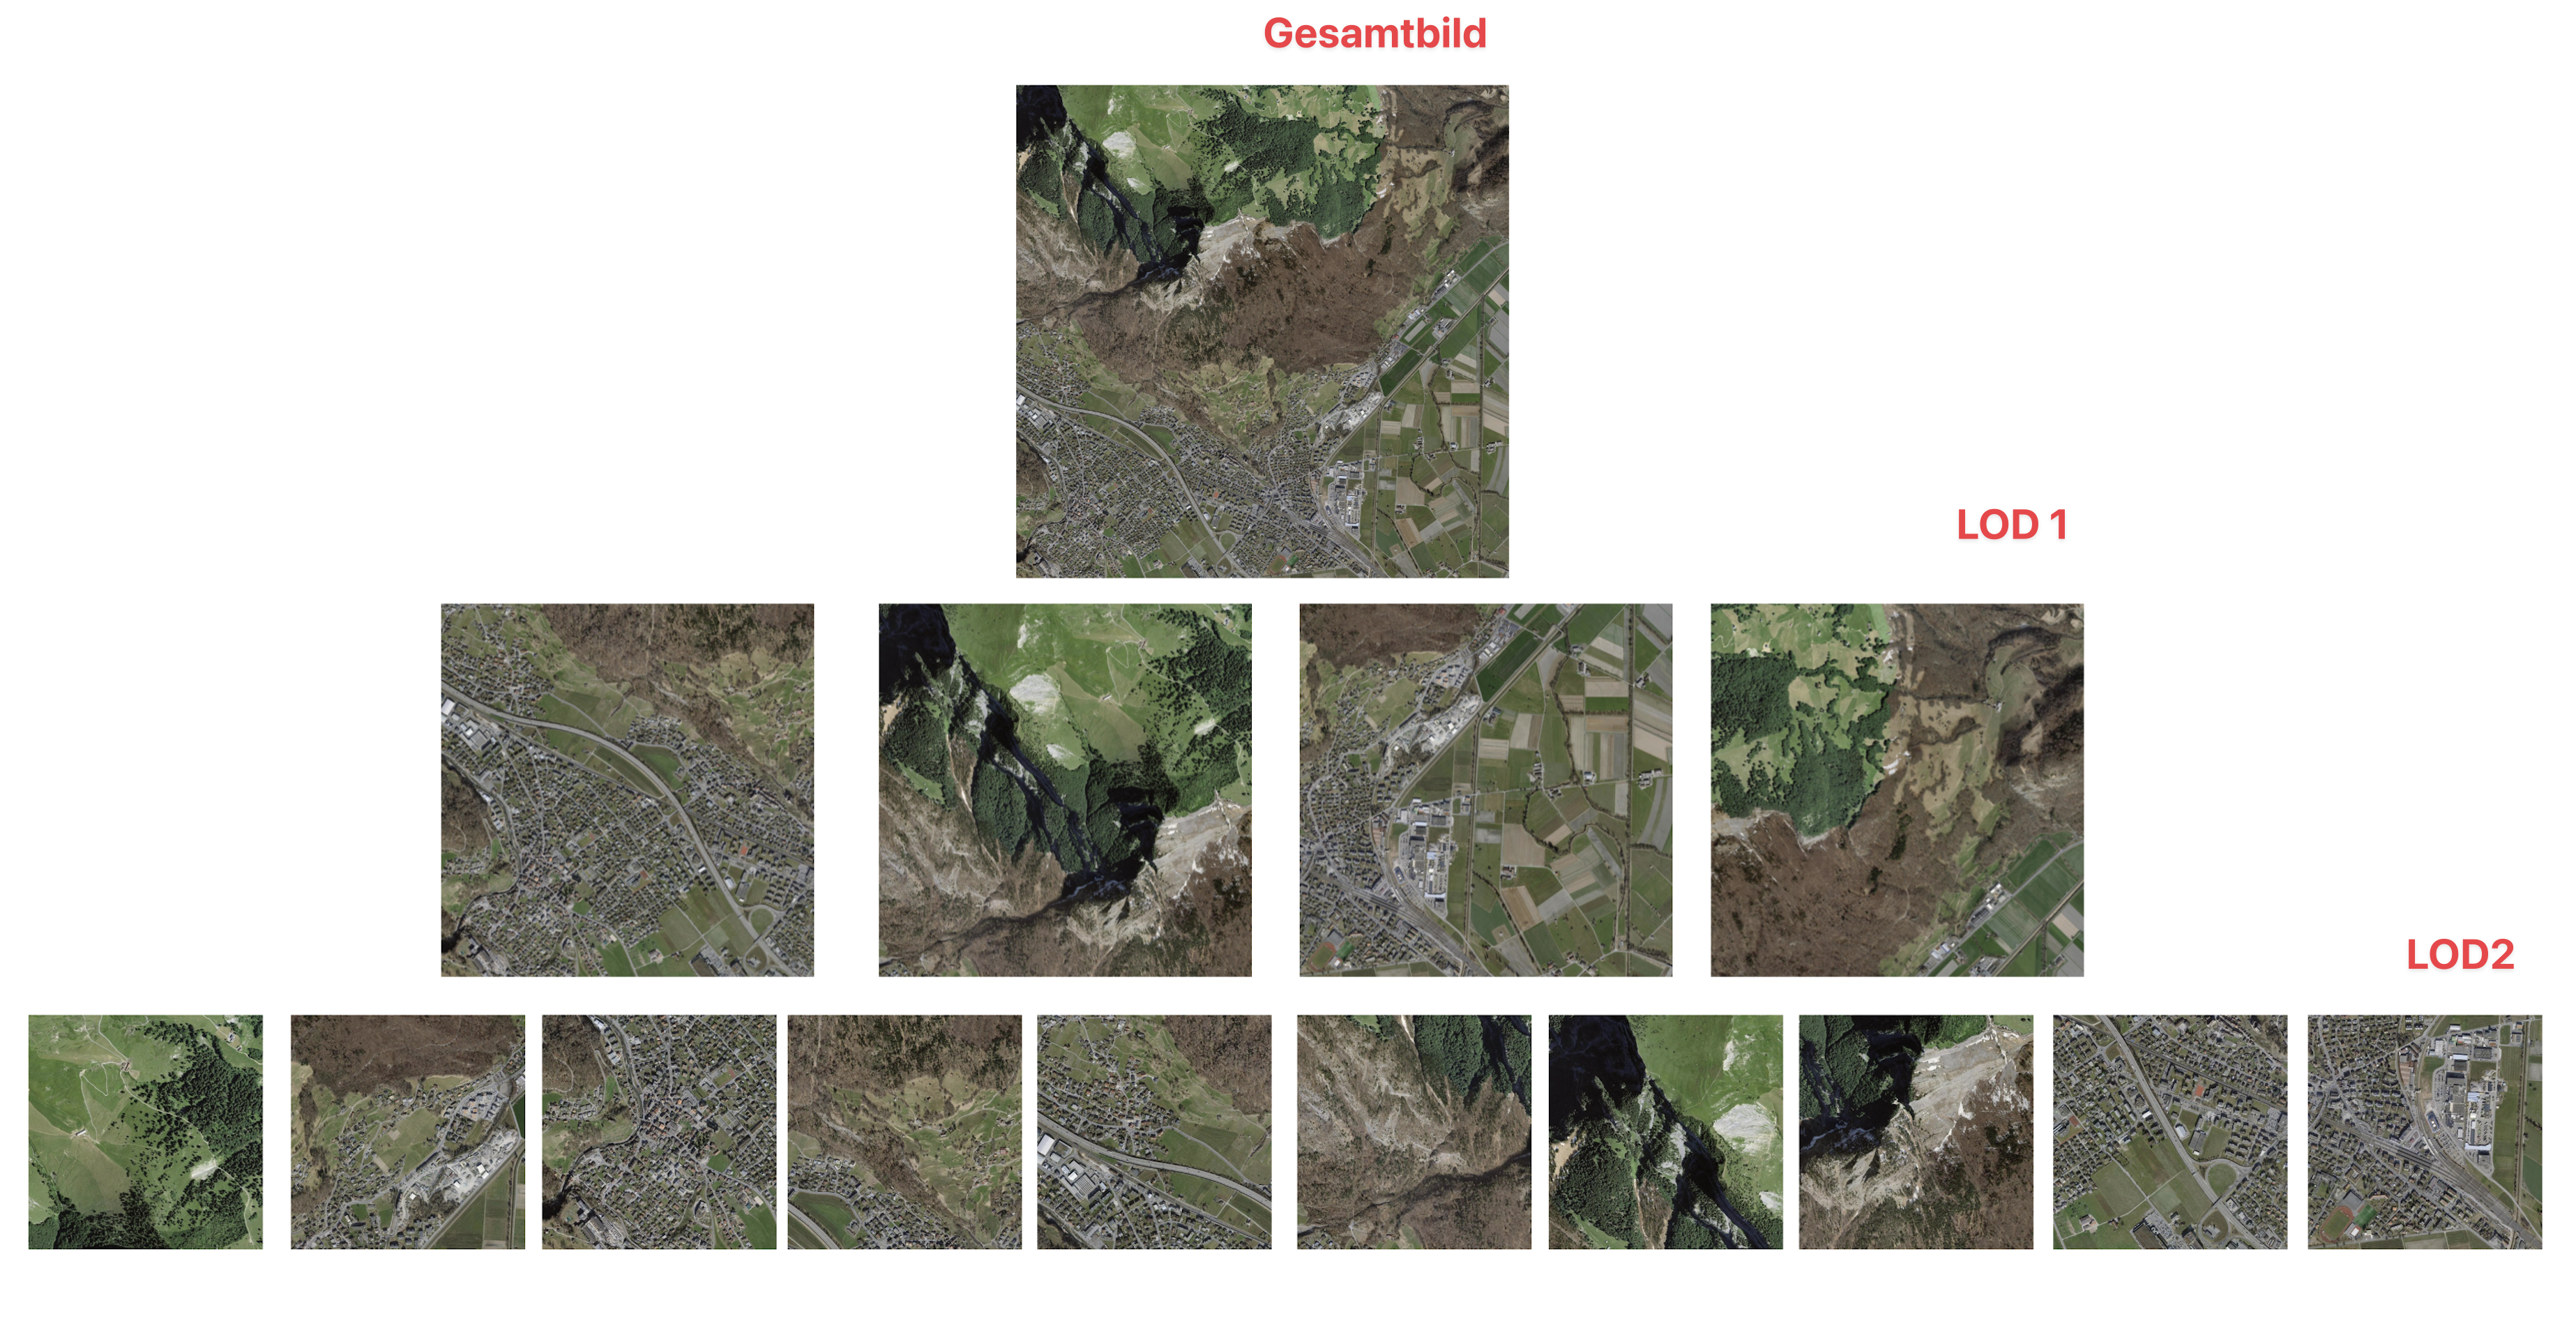
\includegraphics[width=1.0\linewidth]{content/00_assets/zerlegung_in_teilbilder.png}
    \label{fig_textur_teilbilder_quadtree}
\end{figure}

\subsection{Ermittlung des quadratischen Bildausschnitts}
Grafikkarten verarbeiten Texturen mit gleich langen Seiten (500 × 500 Pixel) besonders effizient. Das zusammengesetzte Gesamtbild weist jedoch je nach Region und gewähltem Ausschnitt unterschiedliche Seitenverhältnisse auf. Daher wird das Bild zusätzlich auf einen quadratischen Ausschnitt begrenzt (siehe Abbildung \ref{fig_begrenzung_bildausschnitt}). Dieser Ausschnitt wird so gewählt, dass sich das Gesamtbild vollständig und ohne Restflächen in Tiles unterteilen lässt (siehe LOD 2 in Abbildung \ref{fig_textur_teilbilder_quadtree}) 

\begin{figure}[H]
    \caption{Begrenzung Bildausschnitt (Eigene Darstellung)}
    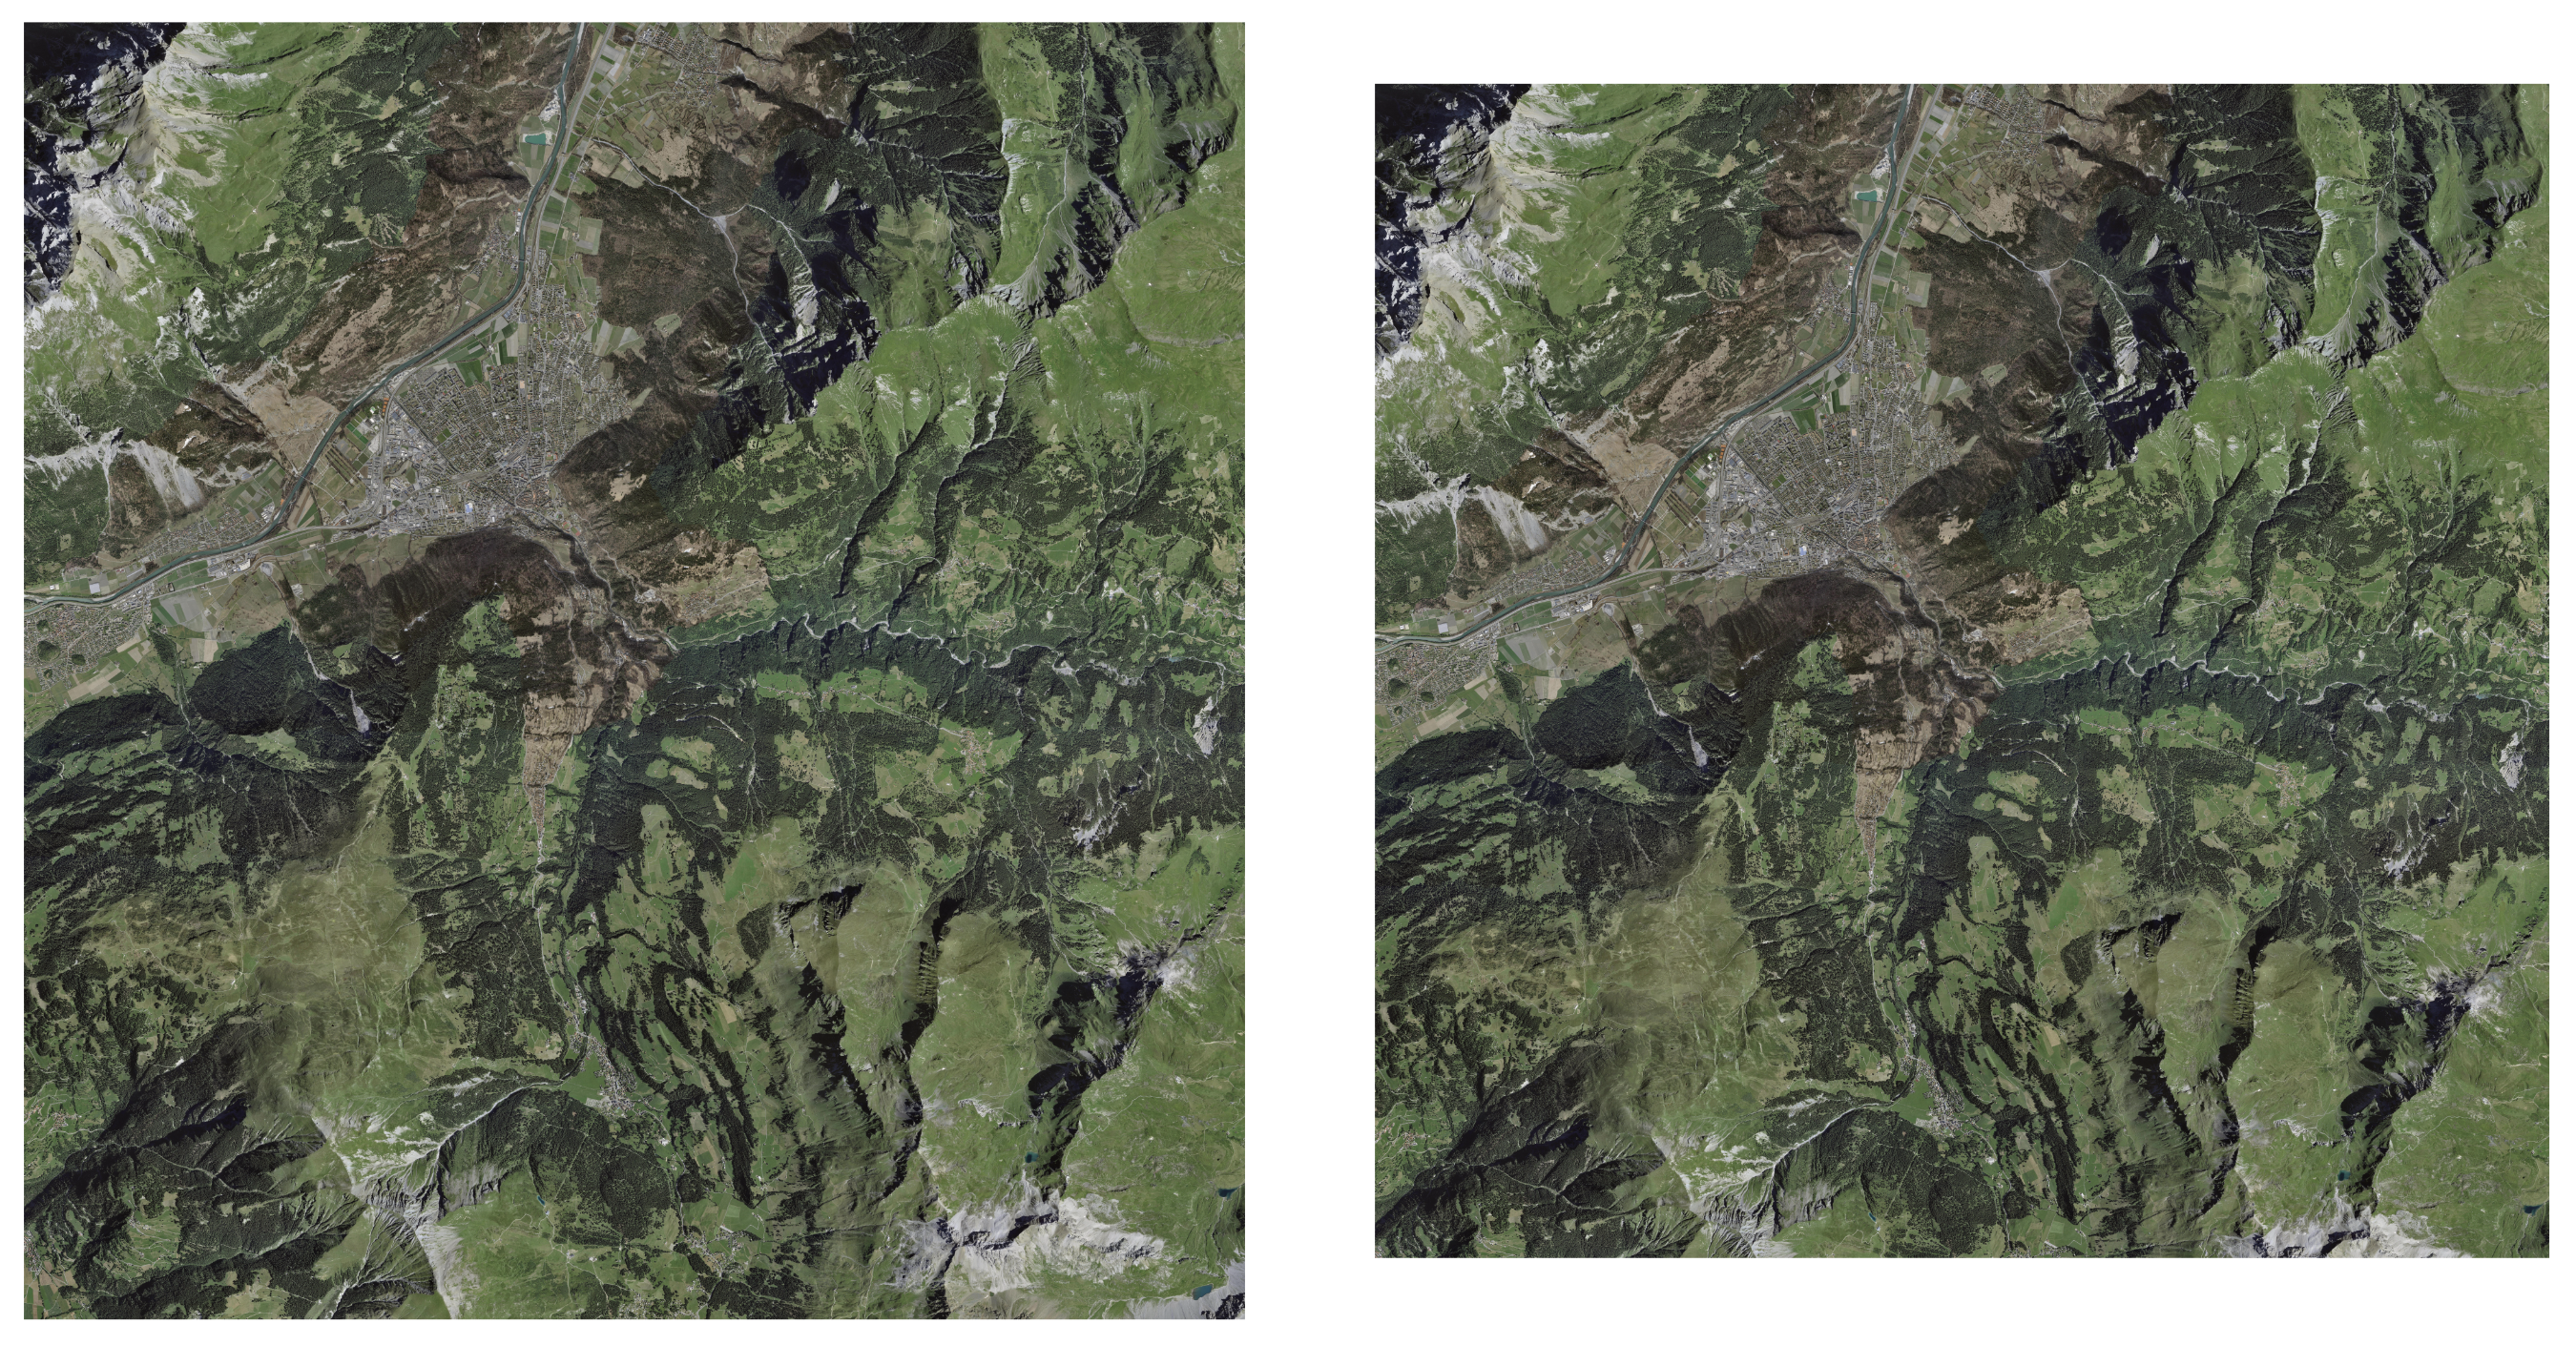
\includegraphics[width=.7\linewidth]{content/00_assets/begrenzung_bildausschnitt.png}
    \label{fig_begrenzung_bildausschnitt}
\end{figure}

\subsection{Automatische Ermittlung der maximalen Baumtiefe}
\label{chap_ermittlung_baumtiefe}
Da sich die Erstellung der Tiles am Quadtree Algorithmus orientiert, lassen sich die maximale Baumtiefe und damit die höchste verfügbare Detailstufe bereits im Vorfeld bestimmen. Zur Veranschaulichung dient folgendes Beispiel: Das Luftbild der Region Sargans besitzt eine Auflösung ($R$) von 2000 auf 2000 Bildpunkten. Bei einer Bodenauflösung von 2m pro Bildpunkt ergibt sich daraus eine effektive Tile-Auflösung ($T$) von 500px ($\frac{1000m}{\frac{2m}{1px}}$) pro km$^2$. Die maximale Baumtiefe ($L_{\max}$) kann auf Basis dieser Parameter mithilfe der Logarithmusfunktion berechnet werden. Für die Region Sargans ergibt sich daraus eine maximale Baumtiefe von 3, was der höchsten darstellbaren Detailstufe entspricht.
\[
L_{\max} = (\log_2\frac{R}{T}) + 1
\]

\subsection{Border Patching}
Auf Basis der extrahierten Höhen- und Bildinformationen lassen sich 3D-Modelle rekonstruieren. Die konkrete Generierung der Geometrie wird in Kapitel \ref{chap_erstellung_geometrie} beschrieben. Werden mehrere dieser Modelle nebeneinander angeordnet, zeigen sich an den Übergängen zwischen benachbarten Tiles sichtbare Risse (siehe schwarze Bereiche in Abbildung \ref{fig_risse_zwischen_3d_modellen}). Diese Artefakte entstehen, da die Höhenwerte entlang der gemeinsamen Kanten nicht exakt mit den Höhenwerten der angrenzenden Tiles übereinstimmen. Infolgedessen weichen die Positionen der Vertices voneinander ab, wodurch sichtbare Lücken in der Geometrie entstehen.
\begin{figure}[H]
    \caption{Risse zwischen 3D Modellen der gleichen Detailstufe (Eigene Darstellung)}
    \includegraphics[width=.3\linewidth]{content/00_assets/risse_zwischen_gleichen_detailstufen.png}
    \label{fig_risse_zwischen_3d_modellen}
\end{figure}

Diese Problematik lässt mit dem sogenannten ``Border Patching'' beheben. Dabei werden an den Kanten der Tiles die Daten der jeweils angrenzenden Nachbartiles übernommen, sodass ein kleiner Überlappungsbereich entsteht. Bereits ein Überlappungsbereich von einem Pixel ist ausreichend, um sichtbare Risse zu vermeiden. Abbildung \ref{fig_border_patching} veranschaulicht diesen Überlappungsbereich in Form roter Linien. Entlang dieser Kanten werden die Höhenwerte der benachbarten Tiles übernommen (von Tile 1 nach Tile 2), wodurch nahtlose Übergänge entstehen.

\begin{figure}[H]
    \caption{Border Patching (Eigene Darstellung)}
    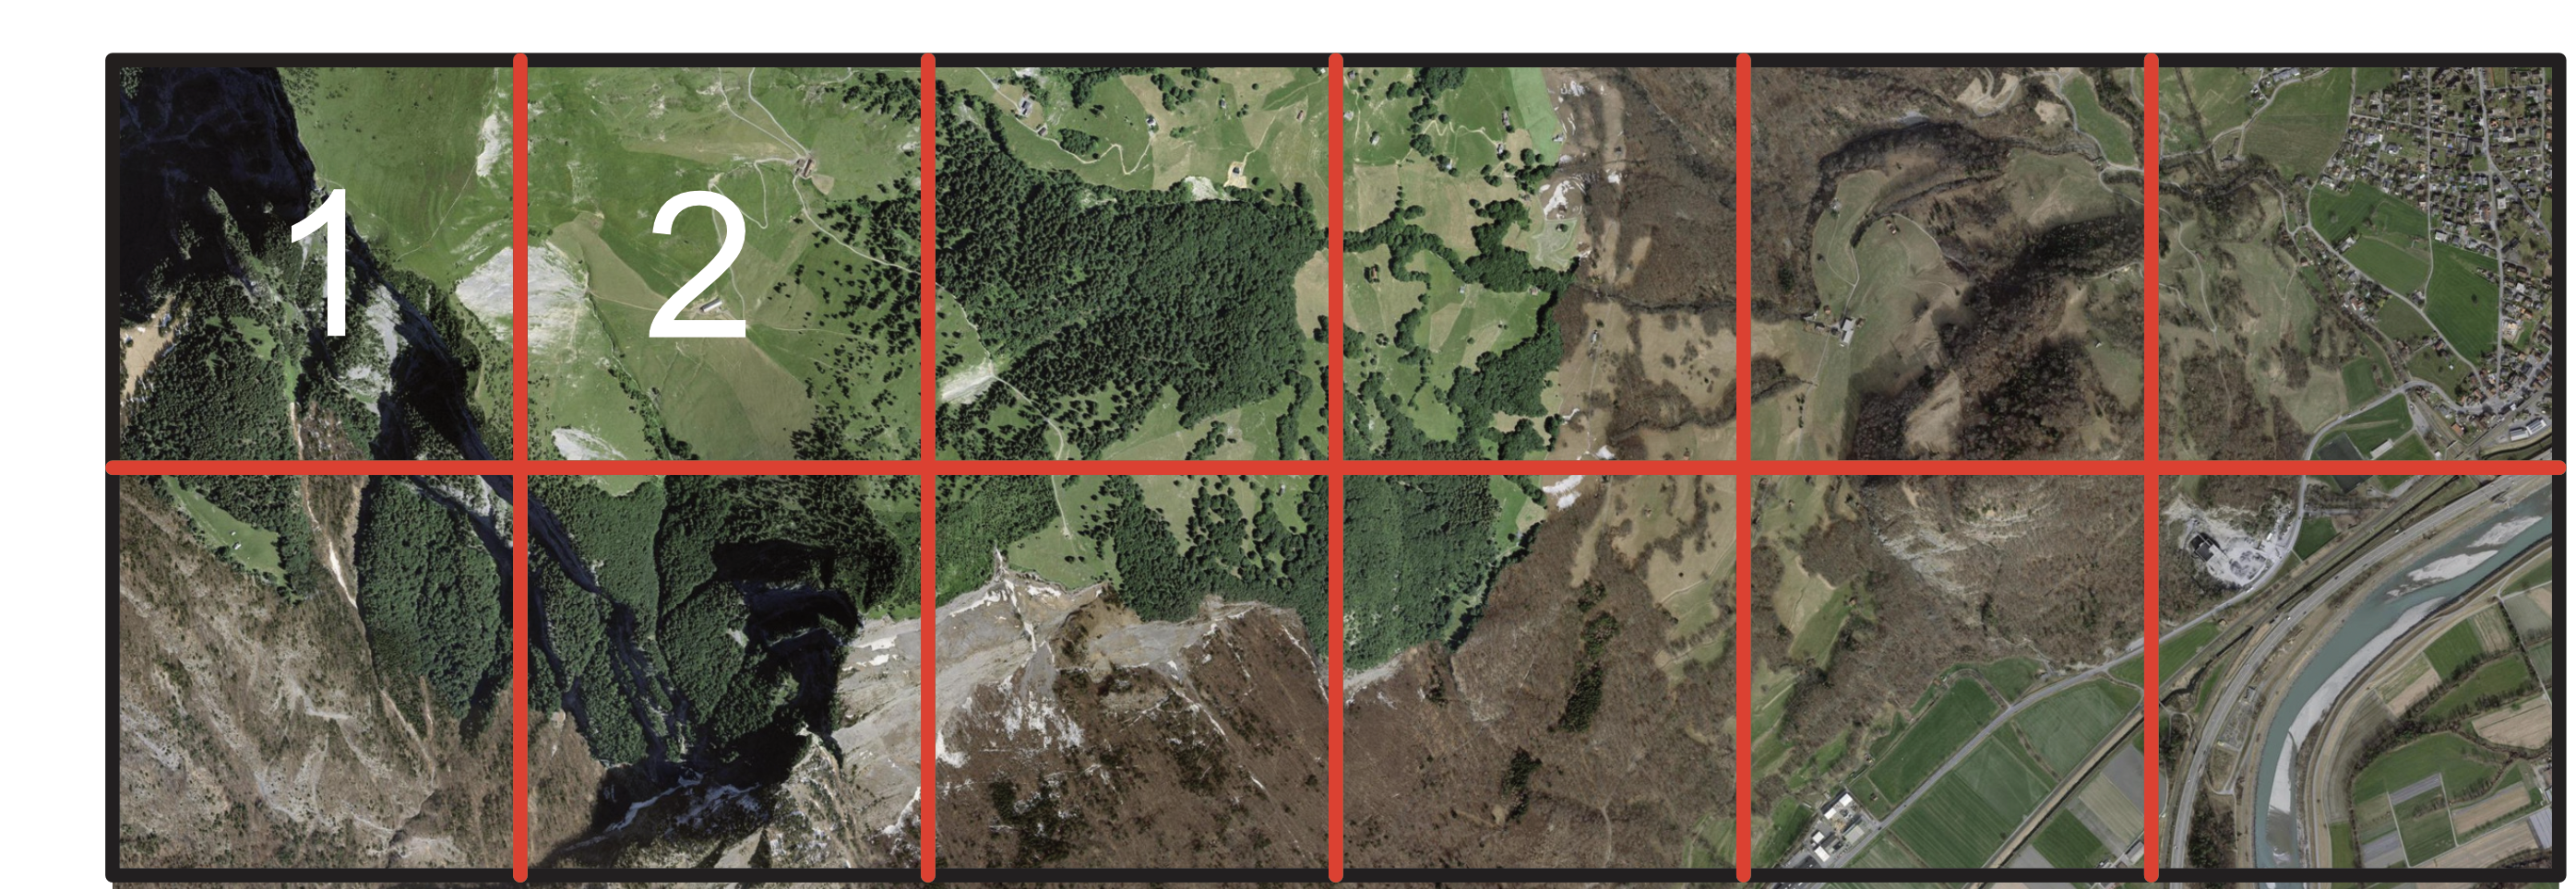
\includegraphics[width=.5\linewidth]{content/00_assets/border_patching.png}
    \label{fig_border_patching}
\end{figure}

\subsection{Relative Geopositionsinformationen}
Das Koordinatensystem von Three.js besitzt einen anderen Ursprung (0/0) als die swisstopo Daten (E=2’600’000 / N=1’200’000). Um die 3D-Modelle in Three.js korrekt zu positionieren, werden daher relative Geopositionsinformationen berechnet. Zunächst wird der Mittelpunkt des Gesamtbildes im LV95-Koordinatensystem bestimmt. Anschliessend wird für jedes Tile der relative Abstand zu diesem Mittelpunkt berechnet und in den zugehörigen Metadaten gespeichert. Auf diese Weise können die 3D-Modelle in Three.js relativ zum Koordinatenursprung platziert werden.

\subsection{Generierung von Metadaten}
\label{chap_generierung_metadaten}
Um wichtige Informationen in Bezug auf die swisstopo Daten nicht zu verlieren, werden entsprechende Metadaten generiert. Diese werden als JSON-Datei gespeichert (siehe Abbildung \ref{fig_ausschnitt_metadaten}) und zur Laufzeit der Webanwendung eingelesen. Tabelle \ref{table_metadata} gibt einen Überblick über die enthaltenen Metadaten sowie deren jeweiligen Verwendungszweck.

\begin{table}[H]
    \caption{Erstellte Metadaten und Verwendungszweck (Eigene Darstellung)}
    \begin{tabularx}{\textwidth} {
        >{\raggedright\arraybackslash}X 
        >{\raggedright\arraybackslash}X}
            \hline
            \textbf{Metadaten} & {Verwendungszweck}  \\
            \hline
            Absolute Geopositionsinformationen (LV95) & LV95 Koordinaten der Tiles \\
            Relative Geopositionsinformationen (LV95) & Relative Positionierung der Tiles zum Three.js Koordinatenmittelpunkt \\
            Maximale Baumtiefe & Limitierungskriterium für den Quadtree Algorithmus \\
            Dateipfade zu den erstellten Bilddateien & Werden zur Laufzeit geladen und bilden die Grundlage für die 3D-Geometrien \\
            \hline
    \end{tabularx}
    \bigbreak
    \label{table_metadata}
\end{table}

\begin{figure}[H]
    \caption{Auszug aus den generierten Metadaten (Eigene Darstellung)}
    \includegraphics[width=.5\linewidth]{content/00_assets/ausschnitt_metadaten.png}
    \label{fig_ausschnitt_metadaten}
\end{figure}

\section{Implementierung}
Dieses Kapitel beschreibt die Implementierung der 3D-Terrainvisualisierung auf Basis des Three.js-Frameworks und der swisstopo-Daten. Zunächst wird erläutert, wie aus den vorverarbeiteten Daten die eigentlichen 3D-Modelle erzeugt werden. Darauf aufbauend werden die eingesetzten Algorithmen sowie begleitende Hilfsvisualisierungen vorgestellt. Abschliessend wird die Implementierung der Steuerungselemente zur freien Navigation im dreidimensionalen Raum beschrieben. Die entwickelte Terrainvisualisierung steht unter der MIT-Lizenz und ist auf GitHub\footnote{\url{https://github.com/yhutter/swiss-terrain-3d}} verfügbar.

\subsection{Erstellung der 3D-Geometrie}
\label{chap_erstellung_geometrie}
Zur Darstellung der Gebirgsgeometrie wird ein Gitternetz aus Punkten verwendet. In Three.js kommt hierfür die sogenannte ``PlaneGeometry'' zum Einsatz, welche eine Ebene im 3D-Raum repräsentiert (siehe Abbildung \ref{fig_threejs_plane_geometry}). Durch eine entsprechende Erhöhung der Segmentierung lässt sich die Auflösung dieser Geometrie beliebig verfeinern.

\begin{figure}[H]
    \caption{Three.js PlaneGeometry \parencite{threejs_beispiel_plane_geometry_2025}}
    \includegraphics[width=.3\linewidth]{content/00_assets/threejs_plane_geometry.png}
    \label{fig_threejs_plane_geometry}
\end{figure}

Um Risse im Terrain an den Übergängen zwischen unterschiedlichen LOD-Stufen zu vermeiden, wird anstelle eines diagonalen Gitters ein sternförmiges Punktmuster verwendet (siehe Abbildung \ref{fig_plane_geometry_star_structure}). In Kombination mit dem sogenannten ``Index-Stitching'' können dadurch sichtbare Risse zwischen den Detailstufen eliminiert werden. Eine detaillierte Erläuterung dieses Verfahrens folgt in Kapitel \ref{chap_quadtree_algorithmus}.

\begin{figure}[H]
    \caption{Gitternetz mit sternförmiger Struktur \parencite[S. 54]{frostbite_terrain_rendering_2007}}
    \includegraphics[width=.3\linewidth]{content/00_assets/geometry_star_pattern.png}
    \label{fig_plane_geometry_star_structure}
\end{figure}

Obwohl Three.js eine Vielzahl vordefinierter 3D-Geometrien bereitstellt, besteht auch die Möglichkeit, eigene Geometrien zu definieren. Hierfür stellt Three.js die Klasse \textit{BufferGeometry} zur Verfügung. Auf dieser Basis wurde eine individuelle Geometrie implementiert, um die gewünschte sternförmige Struktur abzubilden. Wie in Kapitel \ref{chap_render_pipelines} erläutert, setzen sich 3D-Modelle aus Dreiecken zusammen, die wiederum aus einzelnen Punkten, sogenannten Vertices, bestehen. Die Zusammensetzung dieser Punkte zu Dreiecken wird über sogenannte ``Indices'' definiert. Abbildung \ref{fig_create_geometry_with_indices} veranschaulicht diesen Zusammenhang exemplarisch: Zur Erzeugung des Dreiecks $abi$ werden die Punkte $a$, $b$ und $i$ miteinander verbunden. Dieses Verfahren wird für alle weiteren Dreiecke wiederholt, bis die vollständige sternförmige Struktur entsteht. 
\begin{figure}[H]
    \caption{Erstellung der Geometrie mittels Indices (Eigene Darstellung)}
    \includegraphics[width=.7\linewidth]{content/00_assets/erstellung_geometry_mittels_indices.png}
    \label{fig_create_geometry_with_indices}
\end{figure}

Zu diesem Zeitpunkt liegen alle Vertices der Geometrie noch auf einer Ebene. Um daraus ein dreidimensionales Terrain zu erzeugen, werden die Punkte anhand der extrahierten Höhendaten vertikal verschoben. Diese Verschiebung erfolgt im Vertex Shader (siehe Kapitel \ref{chap_render_pipelines}). Zunächst werden die Höhenwerte aus den Graustufenbildern ausgelesen und mithilfe der zuvor berechneten globalen Minimal- und Maximalwerte skaliert. Auf Basis dieses skalierten Höhenwertes werden die Vertices der Geometrie entlang der Höhenachse entsprechend versetzt (siehe Abbildung \ref{fig_verschiebung_punkte_vertex_shader}). Der in Abbildung \ref{fig_verschiebung_punkte_vertex_shader} dargestellte Shadercode ist in der \acrfull{TSL} verfasst. Three.js unterstützt sowohl die WebGL- als auch die WebGPU-Grafikschnittstelle, deren native Shader-Sprachen sich unterscheiden. TSL dient hierbei als Abstraktionsschicht und ermöglicht es, beide Schnittstellen mit einer einheitlichen Programmiersprache anzusprechen. Abhängig vom verfügbaren Hardwaresupport wählt Three.js automatisch die geeignete Grafikschnittstelle aus.

\begin{figure}[H]
    \caption{Verschiebung der Punkte im Vertex Shader (Eigene Darstellung)}
    \includegraphics[width=.9\linewidth]{content/00_assets/positionierung_punkte_vertex_shader.png}
    \label{fig_verschiebung_punkte_vertex_shader}
\end{figure}

\subsection{Texturierung der 3D-Geometrie}
\label{chap_texturierung_3d_geometrie}
Zur Darstellung von 3D-Modellen in Three.js wird neben der Geometrie auch ein sogenanntes ``Material'' benötigt. Während die Geometrie die räumliche Struktur eines Modells beschreibt, bestimmt das Material dessen visuelles Erscheinungsbild. Dieses kann neben Texturen auch Farbwerte sowie weitere Darstellungseigenschaften enthalten. Um einen Würfel in grüner Farbe darzustellen, werden in Three.js eine \textit{BoxGeometry} sowie ein \textit{MeshBasicMaterial} mit der entsprechenden Farbe verwendet (siehe Abbildung \ref{fig_threejs_box}).

\begin{figure}[H]
    \caption{Beispielcode zur Erstellung eines Würfels in Three.js \parencite{threejs_beispiel_box_geometry_2025}}
    \includegraphics[width=.9\linewidth]{content/00_assets/threejs_beispiel_box.png}
    \label{fig_threejs_box}
\end{figure}

Analog zum vorherigen Beispiel kann auch die 3D-Geometrie eines Gebirges mit einer Textur versehen werden. In diesem Fall dienen die orthografisch korrigierten Luftbilder des swissIMAGE-Datensatzes als Texturgrundlage. Die entsprechenden Farbwerte werden im Fragment Shader aus den Bilddaten ausgelesen und zur Darstellung der Oberfläche verwendet (siehe Kapitel \ref{chap_render_pipelines}).

\begin{figure}[H]
    \caption{Ausschnitt rekonstruiertes 3D-Modell auf Basis der swisstopo-Daten (Eigene Darstellung)}
    \includegraphics[width=.5\linewidth]{content/00_assets/texturiertes_3d_modell.png}
    \label{fig_texturiertes_3d_modell}
\end{figure}

\subsection{Quadtree Algorithmus}
\label{chap_quadtree_algorithmus}
Als zentraler Algorithmus kommt ein Quadtree zum Einsatz, da dieser im Vergleich zu Geometry Clipmaps und CDLOD eine einfachere Implementierung erlaubt. Wie in Kapitel \ref{chap_algorithmen} beschrieben, benötigt ein Quadtree ein Kriterium, anhand dessen entschieden wird, wann neue Nodes erzeugt werden. In dieser Arbeit wird hierfür die euklidische Distanz zwischen der Kameraposition und dem Mittelpunkt einer Node herangezogen (siehe Abbildung \ref{fig_quadtree_split_metric}). Zusätzlich wird der Quadtree durch die zuvor berechnete maximale Baumtiefe begrenzt (siehe Kapitel \ref{chap_ermittlung_baumtiefe}). Als Eingabeparameter dienen die Länge und Breite des darzustellenden Gebirges. Zur Laufzeit wird die aktuelle Kameraposition fortlaufend in den Quadtree eingefügt, woraufhin die Abstände zu den einzelnen Nodes berechnet und die Struktur dynamisch angepasst wird.

\begin{figure}[H]
    \caption{Quadtree Kriterium zur Erstellung neuer Nodes (Eigene Darstellung)}
    \includegraphics[width=.8\linewidth]{content/00_assets/quadtree_split_metric.png}
    \label{fig_quadtree_split_metric}
\end{figure}

\subsubsection{Assoziierung zu den Metadaten}
Die einzelnen Nodes des Quadtrees enthalten Informationen über das jeweils abgedeckte räumliche Gebiet sowie über die zugehörige Baumtiefe. Um aus diesen Nodes die entsprechenden 3D-Modelle zu rekonstruieren, werden diese Informationen mit den zuvor erzeugten Metadaten (siehe Kapitel \ref{chap_generierung_metadaten}) assoziiert. Die Zuordnung erfolgt über den Mittelpunkt der Node, der das Zentrum des räumlichen Bereichs beschreibt, sowie über die jeweilige Baumtiefe, welche die Detailstufe festlegt (siehe Abbildung \ref{fig_assoziierung_quadtree_node_metadaten}).

\begin{figure}[H]
    \caption{Assoziierung Quadtree Node zu den Metadaten (Eigene Darstellung)}
    \includegraphics[width=.7\linewidth]{content/00_assets/assoziierung_quadtreenode_metadaten.png}
    \label{fig_assoziierung_quadtree_node_metadaten}
\end{figure}

Der Mittelpunkt einer Node wird aus dem in den Metadaten gespeicherten Bounding-Box-Wert (\textit{bbox\_world\_space}) bestimmt, während die zugehörige Baumtiefe über das Feld \textit{level} definiert ist (siehe Abbildung \ref{fig_ausschnitt_metadaten_tile}). Auf Basis dieser Informationen wird in den Metadaten nach dem passenden Eintrag gesucht und anschliessend das entsprechende 3D-Modell erzeugt. Da sich die Struktur des Quadtrees dynamisch in Abhängigkeit von der Kameraposition verändert, wird zudem sichergestellt, dass nicht mehr benötigte Modelle entfernt werden.
\begin{figure}[H]
    \caption{Ausschnitt Tile Metadaten (Eigene Darstellung)}
    \includegraphics[width=.7\linewidth]{content/00_assets/ausschnitt_metadaten_tile.png}
    \label{fig_ausschnitt_metadaten_tile}
\end{figure}

\subsubsection{Risse zwischen Nodes mit unterschiedlicher Baumtiefe}
\label{chap_visuelle_diskrepanz_zwischen_nodes}
Je nach Baumtiefe erstrecken sich die einzelnen Nodes über einen grösseren Bereich. Für jede Node wird die gleiche sternförmige Grundgeometrie verwendet (siehe Kapitel \ref{chap_erstellung_geometrie}). Treffen Geometrien mit einer unterschiedlichen Baumtiefe aufeinander, entstehen visuelle Diskrepanzen in Form von Rissen (siehe rote Bereiche in Abbildung \ref{fig_visuelle_diskrepanzen_zwischen_unterschiedlichen_lod_leveln}). 
\begin{figure}[H]
    \caption{Visuelle Diskrepanzen zwischen Geometrien mit einer unterschiedlichen Baumtiefe \parencite{frostbite_terrain_rendering_2007}}
    \includegraphics[width=.4\linewidth]{content/00_assets/lod_tjunctions.png}
    \label{fig_visuelle_diskrepanzen_zwischen_unterschiedlichen_lod_leveln}
\end{figure}

Die Risse entstehen, da feinere Geometrien zusätzliche Vertices enthalten, die nicht mit den Vertices der gröberen Geometrien übereinstimmen. Diese zusätzlichen Vertices werden im Vertex-Shader ebenfalls verschoben, was zu sichtbaren Diskontinuitäten in der Geometrie führt (siehe Abbildung \ref{fig_risse_zwischen_3d_modellen_unterschiedlicher_baumtiefe}).
\begin{figure}[H]
    \caption{Risse zwischen 3D-Modellen unterschiedlicher Baumtiefe (Eigene Darstellung)}
    \includegraphics[width=.5\linewidth]{content/00_assets/risse_zwischen_unterschiedlichen_baumtiefen.png}
    \label{fig_risse_zwischen_3d_modellen_unterschiedlicher_baumtiefe}
\end{figure}

\newpage
Zur Behebung dieser Problematik wird das sogenannte ``Index-Stitching'' verwendet, ein Verfahren, das unter anderem in der Frostbite Engine eingesetzt wird. Wie in Kapitel \ref{chap_erstellung_geometrie} beschrieben, legen Indices fest, wie Vertices zu Dreiecken zusammengesetzt werden. Dieses Konzept kann jedoch auch genutzt werden, um bestimmte Vertices gezielt zu überspringen. Hierzu werden mehrere vordefinierte Index-Varianten berechnet, die unterschiedliche Übergangssituationen zwischen benachbarten Geometrien abdecken (siehe Abbildung \ref{fig_frostbite_index_stitching}). Zur Laufzeit wird für jede Geometrie die passende Index-Variante ausgewählt, sodass Risse an den Übergängen vermieden werden.
\begin{figure}[H]
    \caption{Frostbite Engine Index-Stitching \parencite[S. 55]{frostbite_terrain_rendering_2007}}
    \includegraphics[width=.5\linewidth]{content/00_assets/frostbite_index_stitching.png}
    \label{fig_frostbite_index_stitching}
\end{figure}

Zur Auswahl des korrekten Index-Buffers werden für jede Node im Quadtree die benachbarten Nodes ermittelt. Nachbarn mit identischer Baumtiefe werden dabei nicht berücksichtigt. Grenzt eine Node an eine Nachbar-Node mit höherer Auflösung, wird abhängig von der betroffenen Kante der entsprechende Index-Buffer ausgewählt (siehe Abbildung \ref{fig_auswahl_index_stitching}).
\begin{figure}[H]
    \caption{Ermittlung Index-Stitching (Eigene Darstellung)}
    \includegraphics[width=.5\linewidth]{content/00_assets/ermittlung_index_stitching_mode.png}
    \label{fig_auswahl_index_stitching}
\end{figure}

\newpage

Abbildung \ref{fig_wireframe_index_stitching} zeigt eine Wireframe-Ansicht zweier angrenzender Geometrien mit einer unterschiedlichen Baumtiefe. Wie an den Rändern zu erkennen ist, gibt es keine zusätzlichen Vertices mehr und die Geometrien passen korrekt aneinander.
\begin{figure}[H]
    \caption{Wireframe-Ansicht für Index-Stitching (Eigene Darstellung)}
    \includegraphics[width=.4\linewidth]{content/00_assets/index_stitching_wireframe.png}
    \label{fig_wireframe_index_stitching}
\end{figure}

Eine Limitation des Index-Stitching besteht darin, dass sich die Baumtiefe benachbarter Quadtree-Nodes höchstens um eine Stufe unterscheiden darf \parencite[S. 53]{frostbite_terrain_rendering_2007}. Um diese Voraussetzung zu erfüllen, wird der Quadtree entsprechend ausbalanciert.

\subsubsection{Hilfsvisualisierung}
Um sowohl die Korrektheit des Quadtrees als auch der Index-Stitching Methode zu verfizieren wurde eine entsprechende Hilfsvisualisierung implementiert. Die einzelnen Nodes des Quadtrees werden als weisse Linien dargestellt. Nodes, bei denen ein Index-Stitching notwendig ist, sind durch rote Linien gekennzeichnet (siehe Abbildung \ref{fig_hilfsvisualisierung_quadtree_index_stitching}).
\begin{figure}[H]
    \caption{Hilfsvisualisierung für Quadtree und Index-Stitching Überprüfung (Eigene Darstellung)}
    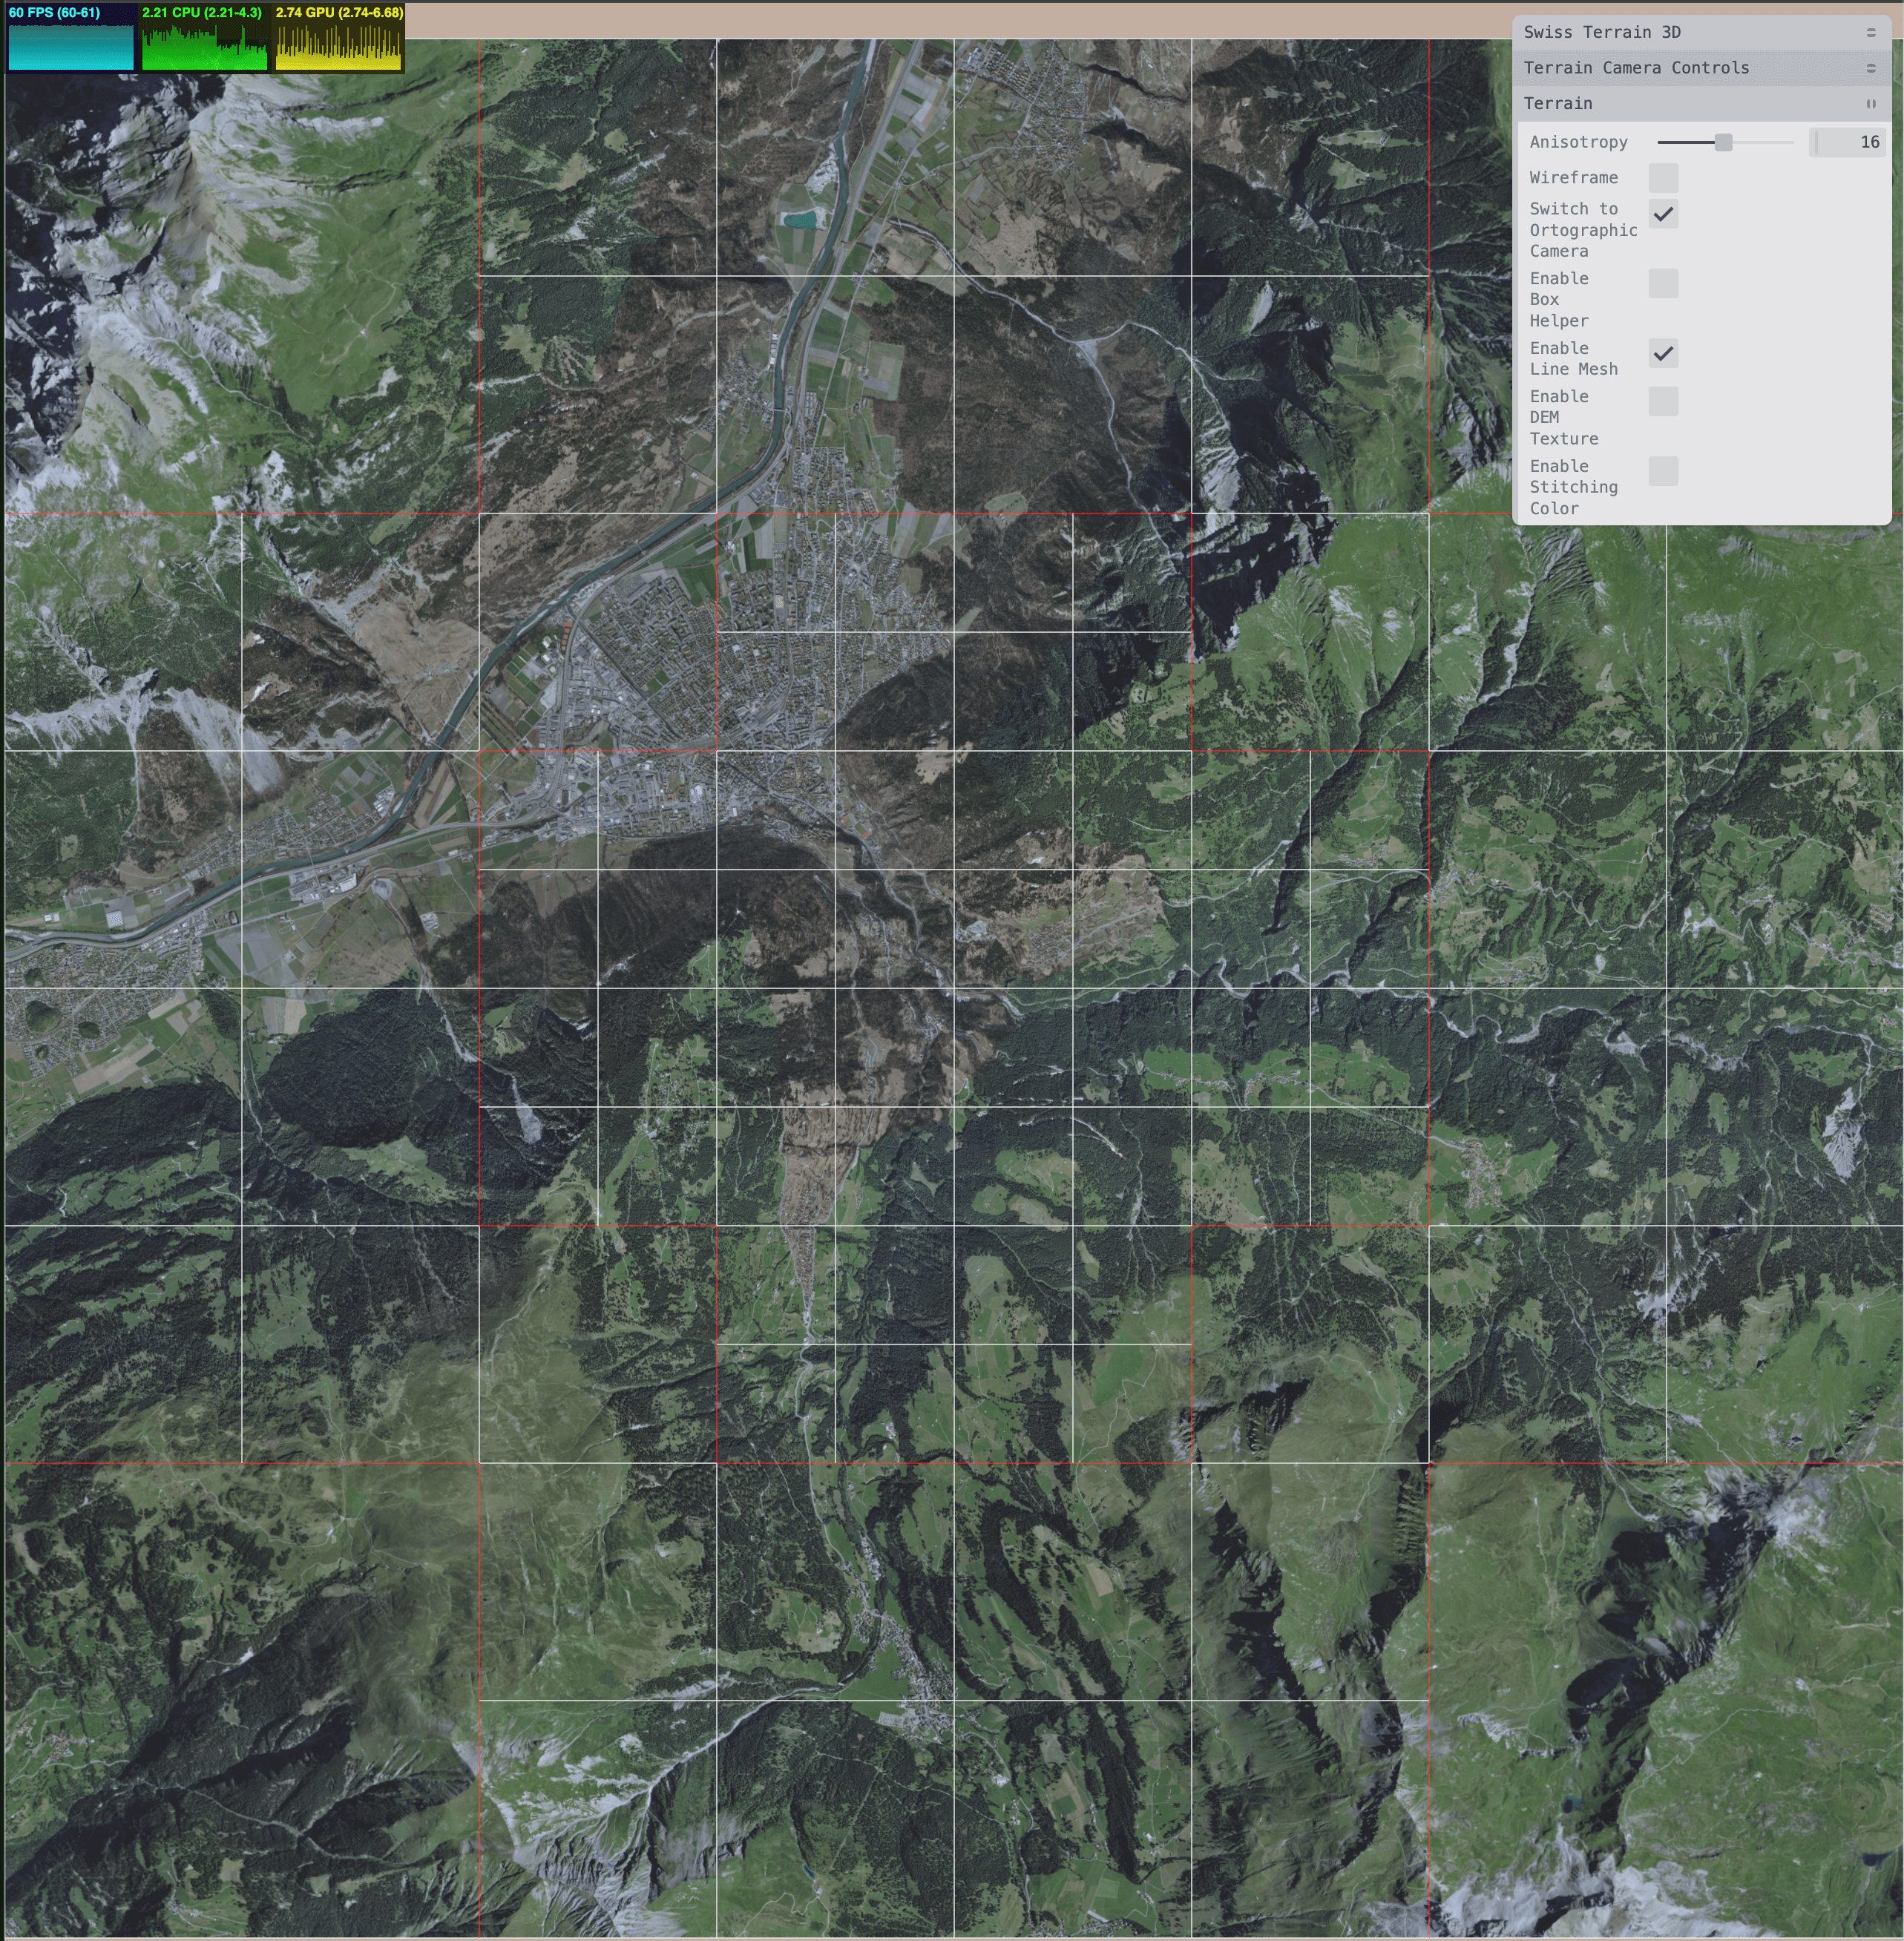
\includegraphics[width=.4\linewidth]{content/00_assets/hilfsvisualisierung_quadtree.png}
    \label{fig_hilfsvisualisierung_quadtree_index_stitching}
\end{figure}

\subsection{Steuerungselemente}
\label{chap_steuerungselemente}
Damit eine freie Bewegung durch das Gebirge möglich ist, müssen entsprechende Steuerungselemente implementiert werden. Der Betrachtungsausschnitt der Visualisierung wird durch eine Kamera definiert. In Three.js stehen verschiedene Arten von Kameras zur Verfügung. Eine ``Perspective Camera'' wird beispielsweise eingesetzt, um Objekte im 3D-Raum darzustellen. Dabei erscheinen die entsprechenden Objekte, abhängig von der Distanz zur Kamera, entsprechend grösser oder kleiner. Die ``Ortographic Camera'' stellt alle Objekte unabhängig von der Distanz gleich gross dar (siehe Abbildung \ref{fig_threejs_cameras}). Aus diesen Gründen wird für die Terrainvisualisierung eine Perspective Camera und für Hilfsvisualisierung eine Ortographic Camera verwendet. 
\begin{figure}[H]
    \caption{Verschiedene Arten von Kameras in Three.js \parencite{threejs_exploring_cameras_2023}}
    \includegraphics[width=.5\linewidth]{content/00_assets/threejs_cameras.png}
    \label{fig_threejs_cameras}
\end{figure}

Mittels Maus und Tastatur können sowohl die Position als auch der Betrachtungswinkel der Kameras verändert werden und erlauben somit eine freie Bewegung durch die Terrainvisualisierung. Tabelle \ref{table_steuerungselemente} zeigt eine Übersicht der Steuerungselemente und deren Auswirkung.
\begin{table}[H]
    \caption{Übersicht über Steuerungselemente und deren Auswirkung (Eigene Darstellung)}
    \begin{tabularx}{\textwidth} {
        >{\raggedright\arraybackslash}X 
        >{\raggedright\arraybackslash}X}
            \hline
            \textbf{Steuerungselement} & {Auswirkung}  \\
            \hline
            W-Taste oder Pfeiltaste nach oben & Bewegung nach vorne \\
            A-Taste oder Pfeiltaste nach link & Bewegung nach links \\
            S-Taste oder Pfeiltaste nach unten & Bewegung nach hinten \\
            D-Taste oder Pfeiltaste nach rechts & Bewegung nach rechts \\
            E-Taste & Bewegung nach oben \\
            R-Taste & Bewegung nach unten \\
            Mausbewegung & Veränderung des Betrachtungswinkels \\
            \hline
    \end{tabularx}
    \bigbreak
    \label{table_steuerungselemente}
\end{table}

\section{Ästhetik}
Three.js bietet zahlreiche Möglichkeiten, die Ästhetik einer 3D-Visualisierung gezielt zu beeinflussen. Ziel dieses Kapitels ist es, einen Überblick über die eingesetzten ästhetischen Anpassungen sowie deren jeweilige Auswirkungen auf die visuelle Darstellung zu geben.

\subsection{High Dynamic Range und Tone Mapping}
\acrfull{HDR} ermöglicht im Kontext digitaler Bilder eine feinere Darstellung des Helligkeitsspektrums. In herkömmlichen Bildformaten sind Farben nur innerhalb eines begrenzten Intensitätsbereichs unterscheidbar. Helle Bildbereiche werden weiss dargestellt, während dunkle Bereiche schwarz erscheinen. Dieser darstellbare Intensitätsbereich wird als Dynamic Range bezeichnet. Da HDR diesen Bereich deutlich erweitert und in feineren Abstufungen abbildet, können Helligkeitsunterschiede präziser dargestellt werden \parencite{hdr_2022}. Abbildung \ref{fig_terrain_hdr_no_hdr} veranschaulicht die resultierenden Kontrastunterschiede.

\begin{figure}[H]
    \caption{Kontrastunterschied der Gebirge mit HDR (links) und ohne (rechts) (Eigene Darstellung)}
    \includegraphics[width=1.0\linewidth]{content/00_assets/terrain_hdr_no_hdr.png}
    \label{fig_terrain_hdr_no_hdr}
\end{figure}

Zur Erstellung von HDR-Bildern existieren mehrere Ansätze. Einerseits können sie synthetisch am Computer erzeugt werden, andererseits lassen sich HDR-Bilder auch aus mehreren Einzelaufnahmen mithilfe spezieller Kamerasensoren berechnen \parencite{hdr_2022}. Zusätzlich stehen spezialisierte Plattformen wie Poly Haven\footnote{\url{https://polyhaven.com/hdris}} zur Verfügung.

Damit die Farbwerte von HDR-Bildern auf dem Bildschirm dargestellt werden können, müssen diese in ein darstellbares Helligkeitsspektrum überführt werden. Hierfür wird das sogenannte ``Tone Mapping'' verwendet. Three.js unterstützt verschiedene Tone-Mapping-Verfahren, die sich jeweils unterschiedlich auf Kontrast und Helligkeitsverteilung auswirken. Abbildung \ref{fig_tone_mapping_threejs} veranschaulicht die Effekte dieser Verfahren auf die finale Darstellung.

\begin{figure}[H]
    \caption{Verschiedene Tone Mapping-Verfahren in Three.js von links nach rechts (kein Tone Mapping, Agx, Filmic, Reinhard) (Eigene Darstellung)}
    \includegraphics[width=.8\linewidth]{content/00_assets/tone_mapping_threejs.png}
    \label{fig_tone_mapping_threejs}
\end{figure}

\subsection{Anisotropy}
Zur Verbesserung der Performance können für Texturen sogenannte ``Mipmaps'' erzeugt werden. Dabei handelt es sich um herunterskalierte Versionen der ursprünglichen Textur (siehe Abbildung \ref{fig_mipmaps}). Abhängig von Betrachtungsabstand und Blickwinkel wählt die Grafikkarte automatisch die jeweils passende Mipmap-Stufe aus. Auf diese Weise werden für weiter entfernte Objekte kleinere Texturversionen verwendet, was den Speicherbedarf reduziert und die Performanz der Visualisierung erhöht \parencite{mipmaps_2023}.

\begin{figure}[H]
    \caption{Mipmaps \parencite{mipmaps_2023}}
    \includegraphics[width=.3\linewidth]{content/00_assets/mipmaps.jpg}
    \label{fig_mipmaps}
\end{figure}

Bei der Verwendung von Mipmaps kann es vorkommen, dass Texturen in grösserer Entfernung unscharf oder nur noch schwer erkennbar dargestellt werden. Um diesem Effekt entgegenzuwirken, kann der Anisotropy-Wert angepasst werden. Dieser legt fest, wie häufig die einzelnen Texel einer Mipmap während der Filterung berücksichtigt werden \parencite{threejs_anisotropy_2025}. Durch eine erhöhte Anisotropie lassen sich verwaschene Texturen, insbesondere bei schrägen Blickwinkeln, deutlich reduzieren (siehe die rot markierten Bereiche A und B in Abbildung \ref{fig_anisotropy}).

\begin{figure}[H]
    \caption{Texturen mit Anisotropy (links) und ohne (rechts) (Eigene Darstellung)}
    \includegraphics[width=1.0\linewidth]{content/00_assets/textur_mit_anisotropy_ohne.png}
    \label{fig_anisotropy}
\end{figure}

\subsection{Procedural Sky}
Das Three.js-Ökosystem stellt zahlreiche Module zur Verfügung, mit denen sich realitätsnahe Visualisierungen umsetzen lassen. Ein Beispiel hierfür ist das Procedural Sky Plugin\footnote{\url{https://github.com/mrdoob/three.js/blob/dev/examples/webgpu_sky.html}}, das die Simulation eines Tag-Nacht-Zyklus ermöglicht. Über verschiedene Parameter, wie die Sonnenposition, kann die Beleuchtung gezielt angepasst und das dargestellte Gebirge in eine realistische Lichtumgebung eingebettet werden. Abbildung \ref{fig_procedural_sky} zeigt den Einfluss unterschiedlicher Sonnenpositionen auf die visuelle Darstellung des Terrains.

\begin{figure}[H]
    \caption{Gebirge mit Procedural Sky Plugin (Eigene Darstellung)}
    \includegraphics[width=1.0\linewidth]{content/00_assets/threejs_procedural_sky.png}
    \label{fig_procedural_sky}
\end{figure}

\subsection{Tweaks}
Die bislang behandelten ästhetischen Elemente verfügen über eine Vielzahl einstellbarer Parameter. Um deren Auswirkungen auf die visuelle Gestaltung nachvollziehen zu können, ist es wichtig, dass diese Parameter während der Laufzeit über geeignete GUI-Elemente angepasst werden können. Für die Verknüpfung von Einstellungsparametern mit grafischen Bedienelementen stehen verschiedene Bibliotheken zur Verfügung. Eine in der Three.js-Community weitverbreitete Lösung ist Tweakpane\footnote{\url{https://tweakpane.github.io/docs/}}. Tweakpane bietet eine Vielzahl unterschiedlicher GUI-Elemente, darunter Slider, Color-Picker und Accordion-Komponenten. Zudem sorgt die Bibliothek für eine einheitliche Darstellung über verschiedene Browser hinweg und ermöglicht eine visuelle Anpassung der Oberfläche mithilfe von Themes\footnote{\url{https://tweakpane.github.io/docs/theming/}}. Der zentrale Vorteil von Tweakpane gegenüber standardmässigen HTML5-GUI-Elementen liegt in der unkomplizierten Verknüpfung von Einstellungsparametern mit den entsprechenden Bedienelementen. Zur Erstellung eines Dropdown-Menüs für die Auswahl des Tone-Mappings müssen lediglich die verfügbaren Optionen sowie die auszuführende Aktion beim Selektieren eines Eintrags definiert werden (siehe Abbildung \ref{fig_tweaks_code}).

\begin{figure}[H]
    \caption{Definitionsstruktur für ein Dropdown in Tweakpane (Eigene Darstellung)}
    \includegraphics[width=.6\linewidth]{content/00_assets/tweaks_beispiel_code.png}
    \label{fig_tweaks_code}
\end{figure}

Diese einfache Handhabung ermöglicht es, schnell neue Bedienelemente für zentrale Parameter zu konfigurieren. Abbildung \ref{fig_tweaks} zeigt eine Auswahl an GUI-Elementen (Tweaks), mit denen verschiedene Aspekte der Terrainvisualisierung in Echtzeit angepasst werden können.

\begin{figure}[H]
    \caption{Tweaks der Terrain-Visualisierung (Eigene Darstellung)}
    \includegraphics[width=.3\linewidth]{content/00_assets/tweaks.png}
    \label{fig_tweaks}
\end{figure}

\section{Performanz}
In diesem Kapitel wird die Leistungsfähigkeit der Terrainvisualisierung evaluiert. Auf dieser Grundlage werden Leistungsengpässe identifiziert und die umgesetzten Optimierungsmassnahmen erläutert. Die Messungen wurden auf einem MacBook Pro M3 Max mit 64 GB Arbeitsspeicher durchgeführt. Als Testgebiet diente der Raum Chur mit einer Ausdehnung von 16km$^2$.

\subsection{Im Vorfeld vorgenommene Optimierungen}
Bereits vor der eigentlichen Messung wurden mehrere Optimierungen umgesetzt. Im Folgenden werden die wichtigsten Massnahmen kurz erläutert.

\subsubsection{Auslagerung des Quadtree-Algorithmus in Web Worker}
Webbrowser führen JavaScript-Code standardmässig in einem einzelnen Thread aus. Rechenintensive Operationen können dadurch die Visualisierung blockieren und zu wahrnehmbaren Verzögerungen führen. Durch den Einsatz von Web Workern lassen sich solche Berechnungen in separate Threads auslagern und im Hintergrund ausführen. Web Worker besitzen keinen Zugriff auf das \acrfull{DOM} des Browsers, weshalb unter anderem das direkte Laden von Texturen nicht möglich ist. Sie eignen sich jedoch für die Auslagerung rechenintensiver Algorithmen, wie beispielsweise des Quadtree-Algorithmus. Auf diese Weise können sowohl die Berechnung als auch das Ausbalancieren des Quadtrees im Hintergrund erfolgen, während sich der Main-Thread auf die Aktualisierung und Darstellung der daraus abgeleiteten 3D-Modelle konzentriert.

\subsubsection{Vorladen der Texturen}
Um ein dynamisches Nachladen der Texturen einzelner Quadtree-Nodes zu vermeiden, werden diese bereits beim Start der Applikation vorgeladen. Zwar führt dies initial zu einer längeren Ladezeit, während der Laufzeit stehen die Texturen jedoch unmittelbar zur Verfügung, sodass Ladeverzögerungen vermieden werden.

\subsubsection{Frustum Culling}
Wie in Kapitel \ref{chap_steuerungselemente} beschrieben, unterstützt Three.js verschiedene Kameratypen, die jeweils ein definiertes Sichtfeld (Frustum) besitzen. Um Rechenleistung zu sparen, werden Objekte ausserhalb dieses Sichtfeldes nicht gezeichnet. Dieses Verfahren wird als ``Frustum Culling'' bezeichnet. Zur Bestimmung, ob sich ein Objekt innerhalb oder ausserhalb des Sichtfeldes befindet, verwendet Three.js sogenannte ``Bounding Spheres''. Diese werden zur Laufzeit für jede Geometrie berechnet. Grundlage hierfür ist eine ``Bounding Box'', also ein dreidimensionaler Bereich, der die jeweilige Geometrie vollständig umschliesst (siehe rote markierte Bereiche in Abbildung \ref{fig_bounding_boxes}).
\begin{figure}[H]
    \caption{Visualisierung der Bounding Box (Eigene Darstellung)}
    \includegraphics[width=.4\linewidth]{content/00_assets/terrain_bounding_boxes.png}
    \label{fig_bounding_boxes}
\end{figure}

\newpage

Die Bounding Box wird aufgrund der globalen Höhenwerte des Gebirges sowie der räumlichen Abdeckung der Quadtree Nodes berechnet. Auf Basis dieses Bereiches kann anschliessend die für das Frustum Culling notwendige Bounding Sphere berechnet werden (siehe Abbildung \ref{fig_berechnung_bounding_box}).

\begin{figure}[H]
    \caption{Berechnung der Bounding Box (Eigene Darstellung)}
    \includegraphics[width=.5\linewidth]{content/00_assets/berechnung_bbox.png}
    \label{fig_berechnung_bounding_box}
\end{figure}

\subsubsection{Vorberechnung der Geometrie}
Die grundlegende Geometrie aller Quadtree-Nodes ist identisch und unterscheidet sich lediglich in ihrer Grösse sowie in der jeweils verwendeten Index-Stitching-Variante (siehe Kapitel \ref{chap_visuelle_diskrepanz_zwischen_nodes}). Dadurch genügen neun vordefinierte Grundgeometrien, jeweils eine pro Index-Stitching-Variante, um das gesamte Gebirge darzustellen. Um aufwendige Berechnungen während der Laufzeit zu vermeiden, werden diese Geometrien bereits beim Start der Applikation vorberechnet. Während der Laufzeit müssen diese anschliessend lediglich den entsprechenden Quadtree-Nodes zugewiesen sowie passend positioniert und skaliert werden.

\subsection{Messung}
Die Messung orientiert sich an den in Kapitel \ref{technologie_anforderungen} definierten Anforderungen. Zur Überwachung der Bildwiederholrate sowie weiterer relevanter Kennzahlen wie CPU- und GPU-Auslastung wird die Bibliothek stats-gl\footnote{\url{https://github.com/RenaudRohlinger/stats-gl}} eingesetzt. Ein wesentlicher Vorteil von stats-gl liegt in der unkomplizierten Integration in das Three.js-Framework. In einem ersten Schritt werden die zu erfassenden Metriken festgelegt (siehe \textit{trackFPS} und \textit{trackGPU} in Abbildung \ref{fig_statsgl}). Anschliessend wird stats-gl initialisiert und periodisch aktualisiert, um die Messwerte während der Laufzeit kontinuierlich zu erfassen.

\begin{figure}[H]
    \caption{Integration von stats-gl in Three.js (Eigene Darstellung)}
    \includegraphics[width=.4\linewidth]{content/00_assets/statsgl.png}
    \label{fig_statsgl}
\end{figure}

Richtig konfiguriert ermöglicht stats-gl die Echtzeitüberwachung der zuvor definierten Metriken. Die Messwerte werden dabei in Form verschiedener Diagramme visualisiert (siehe Abbildung \ref{fig_threejs_statsgl}). Die Auswertung dieser Diagramme zeigt, dass die festgelegten Zielvorgaben hinsichtlich Auflösung und Bildwiederholrate erreicht werden konnten.

\begin{figure}[H]
    \caption{Grafwidgets von stats-gl (Eigene Darstellung)}
    \includegraphics[width=.4\linewidth]{content/00_assets/threejs_statsgl.png}
    \label{fig_threejs_statsgl}
\end{figure}

\subsection{Identifikation von Engpässen}
Während der Navigation durch ein grösseres Gebirge, konkret die Region Chur, konnten insbesondere beim Einsatz des WebGPU-Backends von Three.js kurze Unterbrechungen beobachtet werden. Diese traten jeweils dann auf, wenn neue Geometrien zur Laufzeit erzeugt wurden. Mithilfe der integrierten Browser-Entwicklungswerkzeuge liess sich feststellen, dass rund 60\% der gesamten Laufzeit auf die Methode \textit{build} entfallen (siehe Abbildung \ref{fig_webgpu_build_issue}). 
\begin{figure}[H]
    \caption{WebGPU Engpass in \textit{build} Methode (Eigene Darstellung)}
    \includegraphics[width=.5\linewidth]{content/00_assets/performance_issue_build_method.png}
    \label{fig_webgpu_build_issue}
\end{figure}

Die genannte Methode ist für die Übersetzung des TSL-spezifischen Codes in die jeweilige Shadersprache verantwortlich (GLSL beziehungsweise WGSL). Diese Übersetzung erfolgt auf der CPU und kann bei komplexeren Shadern zu Leistungsengpässen führen. Beim WebGL-Backend entfällt dieser Schritt, da der Shadercode direkt in GLSL geschrieben wird. Ein weiterer Engpass, der sowohl im WebGPU- als auch im WebGL-Backend beobachtet wurde, ist das Dekodieren von Bilddateien. Wie in Abbildung \ref{fig_performance_issue_image_decode} dargestellt, werden im WebGL-Backend rund 40\% der gesamten Ausführungszeit für diesen Prozess aufgewendet.

\begin{figure}[H]
    \caption{Dekodieren der Bilddateien (Eigene Darstellung)}
    \includegraphics[width=.8\linewidth]{content/00_assets/performance_issue_image_decode.png}
    \label{fig_performance_issue_image_decode}
\end{figure}

\subsection{Optimierungen}
Zur Behebung der Übersetzungsproblematik wurde entschieden, das WebGL-Backend anstelle des WebGPU-Backends einzusetzen. Three.js unterstützt den Wechsel des Grafik-Backends, sodass grosse Teile wiederverwendet werden konnten. Lediglich der Shadercode musste im Zuge der Umstellung von TSL auf GLSL angepasst werden (siehe Abbildung \ref{fig_vertex_shader_glsl_tsl}).
\begin{figure}[H]
    \caption{Unterschiede zwischen GLSL und TSL Code (Eigene Darstellung)}
    \includegraphics[width=.6\linewidth]{content/00_assets/terrain_vertex_shader_glsl_tsl.png}
    \label{fig_vertex_shader_glsl_tsl}
\end{figure}

Zur Beseitigung des Dekodierungsengpasses wurde ein speziell für die Grafikkarte optimiertes Texturformat namens \acrfull{KTX}-Format\footnote{\url{https://github.khronos.org/KTX-Specification/ktxspec.v2.html}} eingesetzt. KTX-Texturen liegen bereits in einem für die GPU geeigneten Format vor und müssen nicht mehr zur Laufzeit dekodiert werden. Zu diesem Zweck wurde die Datenvorverarbeitung angepasst, sodass die Texturen zusätzlich im optimierten KTX-Format erzeugt werden.

\subsubsection{Zukünftige Optimierungsmöglichkeiten}
\label{chap_future_optimizations}
Mithilfe von Analysewerkzeugen wie SpectorJS\footnote{\url{https://spector.babylonjs.com}} lässt sich jedes einzelne Bild detailliert auf der Grafikhardware untersuchen. Dabei zeigte sich, dass für jede Geometrie ein eigener Draw Call an die Grafikkarte gesendet wird. Für die Region Chur sind somit rund 89 Draw Calls erforderlich (siehe Abbildung \ref{fig_spectorjs_draw_calls}). Diese Anzahl steigt mit der Zahl der Quadtree-Nodes und damit mit der Grösse des dargestellten Gebirges. Insbesondere auf leistungsschwächeren Endgeräten, wie etwa Smartphones, kann dies zu spürbaren Leistungsengpässen führen.

\begin{figure}[H]
    \caption{SpectorJS - Anzahl Draw Calls für Region Chur (Eigene Darstellung)}
    \includegraphics[width=.3\linewidth]{content/00_assets/spectorjs_draw_calls.png}
    \label{fig_spectorjs_draw_calls}
\end{figure}

Three.js bietet mit dem sogenannten ``Instance Rendering'' eine effektive Lösung für dieses Problem. Mit diesem Verfahren lassen sich viele identische Geometrien innerhalb eines einzigen Draw Calls darstellen. Voraussetzung ist, dass alle Instanzen dieselbe Grundgeometrie verwenden (siehe Abbildung \ref{fig_threejs_instance_rendering}). Da für die Terrainvisualisierung lediglich neun unterschiedliche Geometrievarianten benötigt werden, kann die Anzahl der erforderlichen Draw Calls auf diese Weise deutlich reduziert werden.

\begin{figure}[H]
    \caption{Three.js Instance Rendering \parencite{threejs_instance_rendering_2025}}
    \includegraphics[width=.4\linewidth]{content/00_assets/threejs_instance_rendering.png}
    \label{fig_threejs_instance_rendering}
\end{figure}
